% arara: pdflatex: { synctex: yes }
% arara: makeindex: { style: ctuthesis }
% arara: bibtex

% The class takes all the key=value arguments that \ctusetup does,
% and a couple more: draft and oneside
\documentclass[twoside]{ctuthesis}
\usepackage[toc]{appendix}
\usepackage{graphicx}
\usepackage{subfig}
\usepackage{svg}
\usepackage{placeins}
\usepackage[capposition=bottom]{floatrow}
\usepackage{listings, listings-rust}
\usepackage{multirow}
\usepackage{adjustbox}

\PassOptionsToPackage{hyphens}{url}
\usepackage[pdftex,
            pdfauthor={Jiří Maňák},
            pdftitle={Sensor Network for Smart Agriculture}
			]{hyperref}

\ctusetup{
	preprint = \today,
	mainlanguage = english,
	titlelanguage = english,
	otherlanguages = {czech},
	title-czech = {Senzorová síť pro Smart Agriculture},
	title-english = {Sensor Network for Smart Agriculture},
%	subtitle-czech = {},
%	subtitle-english = {},
	doctype = B,
	faculty = F3,
	department-czech = {Katedra meření},
	department-english = {Department of Measurement},
	author = {Jiří Maňák},
	supervisor = {prof. Ing. Radislav Šmíd, Ph.D.},
	supervisor-address = {Praha, Technická 1902/2, místnost: A3-324},
%	supervisor-specialist = {},
%	fieldofstudy-english = {},
%	subfieldofstudy-english = {},
%	fieldofstudy-czech = {},
%	subfieldofstudy-czech = {},
	keywords-czech = {Senzorová síť, LoRa, Jazyk Rust},
	keywords-english = {Sensor Network, LoRa, The Rust Language},
	day = 21,
	month = 5,
	year = 2024,
	specification-file = {sub/thesis-specification.pdf},
%	front-specification = true,
%	front-list-of-figures = false,
%	front-list-of-tables = false,
%	monochrome = true,
%	layout-short = true,
}


\ctuprocess

\addto\ctucaptionsczech{%
\def\supervisorname{prof. Ing. Radislav Šmíd, Ph.D.}%
\def\subfieldofstudyname{Kybernetika a Robotika}%
}

\ctutemplateset{maketitle twocolumn default}{
	\begin{twocolumnfrontmatterpage}
		\ctutemplate{twocolumn.thanks}
		\ctutemplate{twocolumn.declaration}
		\ctutemplate{twocolumn.abstract.in.titlelanguage}
		\ctutemplate{twocolumn.abstract.in.secondlanguage}
		\ctutemplate{twocolumn.tableofcontents}
		\ctutemplate{twocolumn.listoffigures}
	\end{twocolumnfrontmatterpage}
}

\lstset{language=Rust, style=boxed}

\newcommand{\code}[1]{\lstinline{#1}}
\newcommand{\link}[2]{\href{#1}{#2}\footnote{#1}}

\setlength{\parskip}{1.5ex plus 0.2ex minus 0.1ex}

% Abstract in Czech
\begin{abstract-czech}
Tato bakalářská práce se zabývá vývojem bezdrátového senzoru pro měření vlhkosti půdy, který je užitečný pro efektivní hospodaření s vodními zdroji v zemědělství, zahradnictví a domácnostech. Výsledkem práce jsou dva hardwarové komponenty, univerzální modul s podporou LoRa rozhraní a senzor vlhkosti půdy, založený na kapacitním měření objemového obsahu vody. Modul, postavený na čipu STM32WLE, obsahuje integrovanou nevolatilní paměť pro záznam dat a aktualizace firmwaru, je kompaktní, má nízkou spotřebu a univerzální podporu I/O. Firmware modulu je implementován v programovacím jazyce Rust. Experimentem byla oveřena stabilní komunikace modulu na vzdálenosti přesahující jeden kilometr.
\end{abstract-czech}

% Abstract in English
\begin{abstract-english}
This thesis examines the development of a wireless sensor for soil moisture sensing, crucial for efficient water resource management in agriculture, horticulture, and domestic settings. Outcome of the work are two hardware components, a general purpose LoRa module and the soil moisture sensor, based on capacitive volumetric water content measurement. The module, built on the STM32WLE System on a Chip, features integrated non-volatile memory for data logging and firmware updates, compact size, low power consumption, and versatile I/O support, its firmware is implemented in the Rust language. Field tests confirmed the module's stable communication over distances exceeding one kilometer, demonstrating its effectiveness and potential for broader applications.
\end{abstract-english}

% Acknowledgements / Podekovani
\begin{thanks}
I would like to express gratitude to those who helped and supported me during the creation of this thesis.

First and foremost, I would like to thank my supervisor, Prof.~Radislav~Šmíd, for his insights, positive attitude, ideas and the material support.

Also my partner, Bc.~Diana~Varšíková, for her support, counsel of the visualizations and the final review pass.

Lastly, huge thanks goes to Ing.~Tomáš~Kořínek and Ing.~Jan~Spáčil from the department of electromagnetic field for their willingness, provided access to the instruments and overall great company.
\end{thanks}

% Declaration / Prohlaseni
\begin{declaration}
\noindent I hereby declare that I have independently authored the submitted thesis and have cited all the sources used.
\vspace{1em}
\hrule
\noindent Prohlašuji, že jsem předloženou práci vypracoval samostatně, a že jsem uvedl veškerou použitou literaturu.
\begin{flushright}
V Praze \ctufield{day}.~května~\ctufield{year}
\end{flushright}
\end{declaration}


\begin{document}

\maketitle

\ctutemplate{specification.as.chapter}

\chapter{\label{chapter:introduction}Introduction}
%!TEX ROOT=main.tex

With the upward trend in global temperatures, the world is witnessing an increased scarcity of water resources. This environmental shift poses a significant challenge to traditional farming practices, which are heavily reliant on predictable weather patterns and stable water supply. 

``\emph{Over 60\% of European soils are unhealthy and scientific evidence shows that soils are further degrading due to unsustainable management of the land, sealing, contamination and overexploitation, combined with the impact from climate change and extreme weather events. [...] The loss of these essential soil ecosystem services costs the EU at least 50 billion euro per year.}'', Soil health - European Commission \cite{european_commission_soil_2024}.

In the face of these challenges, the adoption of smart agriculture technologies, emerges as a vital strategy. These technologies offer the potential to transform agricultural practices by optimizing water usage, improving crop yields, and ensuring sustainable farming operations.

This project aims to develop a sensor network that is not only reliable and easy to maintain but also versatile enough to be applied across various contexts - from small--scale home gardens to medium--sized agricultural fields and regional deployments. 

The technical challenges will be the primary focus of this work, and since many of the requirements for a reliable remote sensing solution are common amongst other applications, it will also venture into those, especially in the initial architectural and design stages. 

\section{Goals}
Many options exist when it comes to transferring sensor data over long distances. For this work, the LoRa technology was selected for its unique blend of long-range (orders of 1 to 10 km in favorable conditions), albeit relatively slow (0.3 to 50 kbit \cite{semtech_corporation_sx12612_2024}), data transfer, with very low power consumption (5 mA receiving \cite{semtech_corporation_sx12612_2024}), global availability and general fit for the purpose.

Furthermore, an over--the--air (OTA) firmware update capability will be explored, a feature not commonly found in LoRa nodes. In the case of soil moisture sensors, an update can bring support for additional soil types, improve the accuracy or prolong the battery life. It also, crucially, allows this to happen without any operator intervention and transforms a one-shot solution, which once obsolete is replaced completely, into one that is, over time, able to support more sensors and features with minimal downtime \cite{mobility_connected_what_2024,noauthor_android_2024,bucklin_brown_over--air_2024}.

A custom hardware solution will need to be developed in order to support OTA updates. Chapter \ref{chapter:architecture} in particular will make a point as to why this is necessary by compiling the hardware requirements and assessing the existing solutions currently available on the market. 

This hardware solution will consist of two pieces - a general purpose LoRa module (the ``LoRa module'' from now on) capable of OTA updates and a soil moisture sensor, which integrates the LoRa module into the specialized application.

To implement the sensing, its configuration, status reporting and the update capability, a custom protocol will be developed atop the LoRa physical layer. This will make the system self--sufficient, but may limit the deployment options. However, the system could also be made compatible with the majority of commercial LoRaWAN networks in the future, if needed.

Lastly, on the note of autonomy and minimal maintenance, individual nodes should be power--efficient enough to be powered by a small built--in battery augmented by a solar panel, to achieve a ``set and forget'' deployment. 

The system will be evaluated based on its performance in the field by conducting a range test in actual operating conditions and its sensor's ability to be powered by solar panel will be tested on a prototype unit.

\chapter{\label{chapter:prior}Prior Art}
%!TEX ROOT=main.tex

\section{Soil water content}
Soil is made up of a solid phase of minerals and organic matter, and the pours in-between the solids, which hold gasses and water \cite{paul_soil_2007}. The total amount of moisture is the sum of the moisture contained inside the solids (in intra-aggregate pore space) and the space around the solids (inter-aggregate pore space) \cite{myjove_corporation_determination_2024}. This work will not distinguish between the two for simplicity.

\subsection{Definition}
Soil water or moisture content is a ratio, which ranges from 0, meaning completely dry, to the value of material porosity at saturation \cite{webster_humidity_1998}. It expresses the quantity of water contained in the soil. We can measure it by mass (gravimetric method) or by volume , as depicted in Figure \ref{fig:soil-phase-diagram}.

We can express this mathematically for volumetric content (VWC) as
\begin{equation}
    \label{equation:volumetric-content} \theta = \dfrac{V_w}{V_s + V_w + V_a}
\end{equation}
where $V_w$ is the volume of water and $V_s + V_w + V_a$ is the total volume of the soil sample including contained air. Likewise, gravimetric water content (GWC) is defined as
\begin{equation}
    \label{equation:gravimetric-content} u = \dfrac{m_w}{m_s}
\end{equation}
where $m_w$ is the mass of the water and $m_s$ is mass of all solids in the sample \cite{edaphic_scientific_pty_ltd_how_2024}.

\begin{figure}
    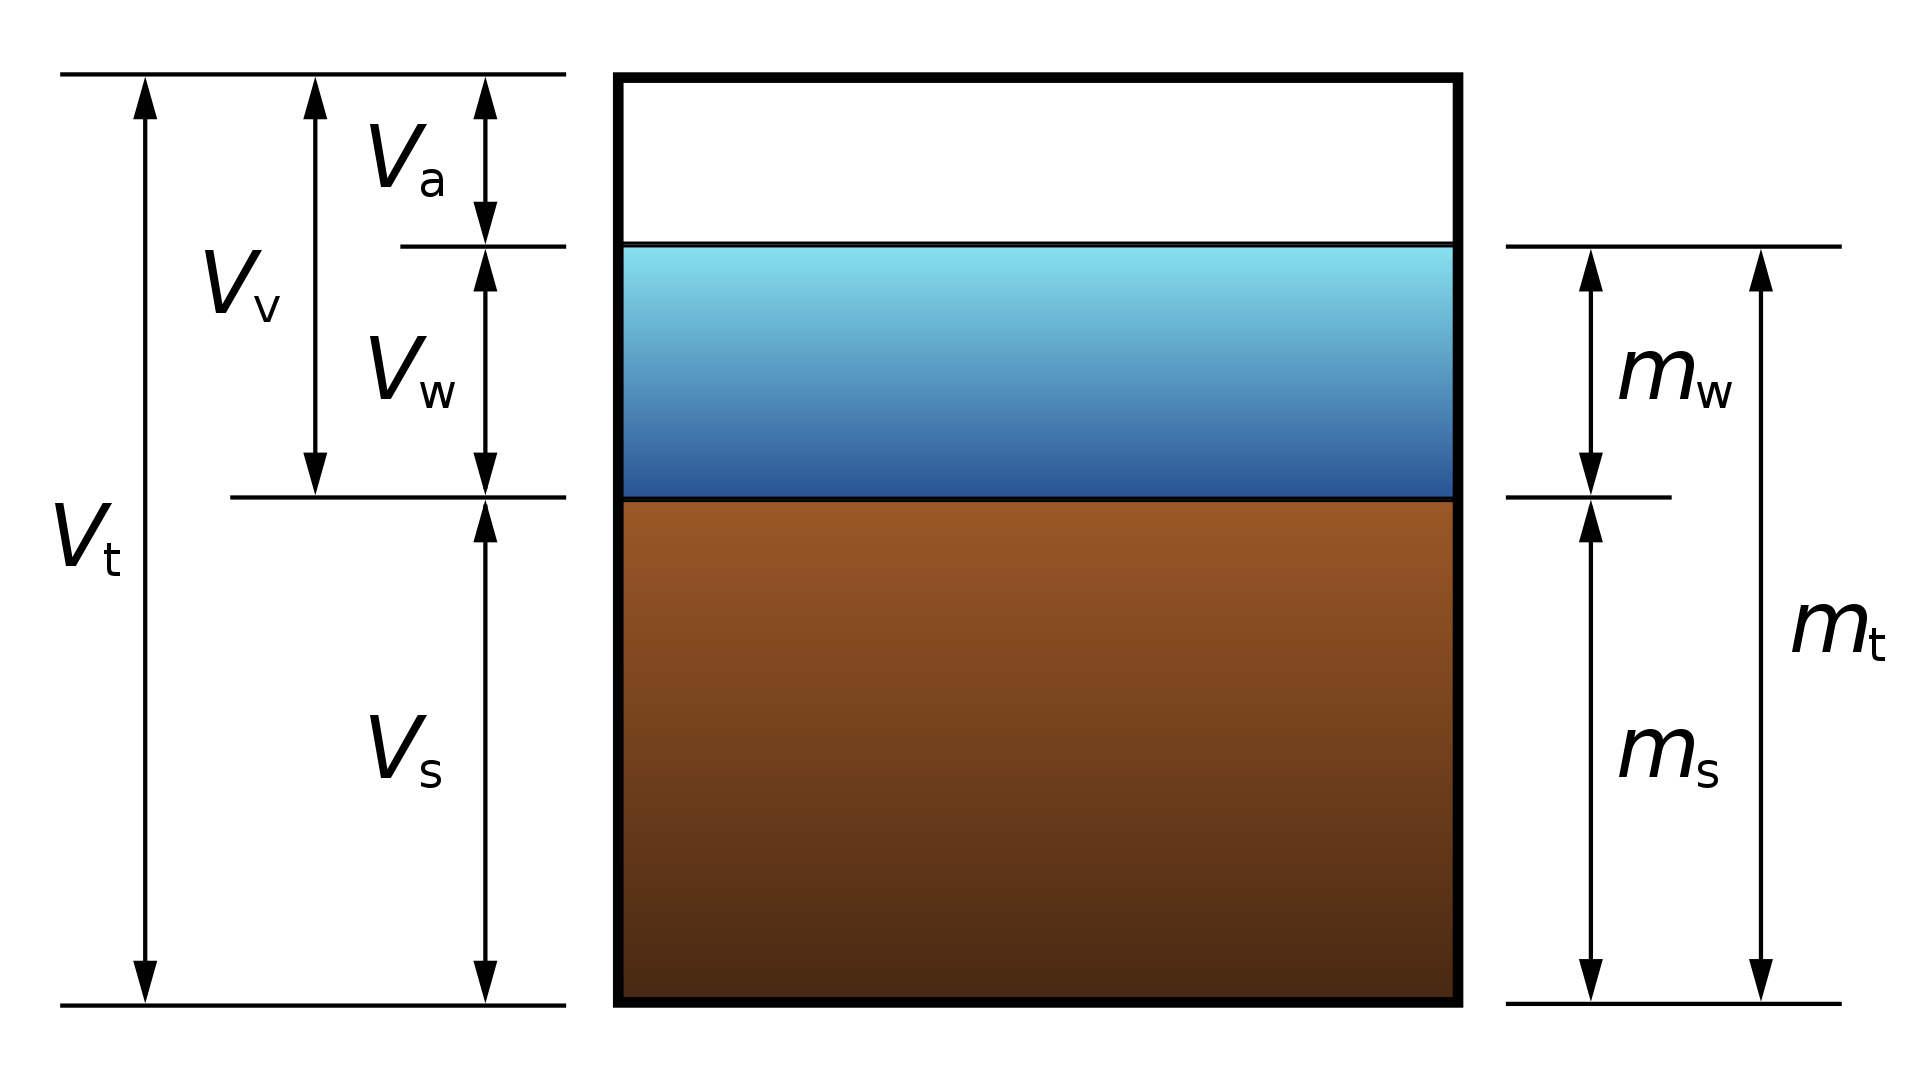
\includegraphics[width=.5\textwidth]{fig/soil-phase-diagram.png}
    \caption{\label{fig:soil-phase-diagram} Soil composition by volume and mass \cite{noauthor_water_2023}}
\end{figure}

\subsection{Methods of measurement}
\subsubsection{Drying the soil}
Drying the soil sample in a drying oven is a direct method of measurement and is used as the reference method \cite{webster_humidity_1998}. By weighing the sample and also measuring its volume, then doing that again after drying, it is possible to very accurately measure both the volumetric and the gravimetric water content both at the same time.

The procedure involves gathering a known quantity of the sample, ranging from 30 grams to 5 kg, depending on the fines of the particles, heating it up and drying it at 65 to 110 degrees Celsius until the weight stops decreasing \cite{department_of_sustainable_natural_resources_soil_2024,myjove_corporation_determination_2024, paul_soil_2007}.

Since direct methods of measurement of soil moisture content are impractical for field use, we will focus on indirect methods next.

\subsubsection{Geophysical methods}
Geophysical methods exploit other properties of water contained in the soil to approximate the VWC, such as its conductivity, dielectric constant or interaction with neutrons. These methods are thus indirect and subject to inaccuracy if wrong assumptions are used \cite{webster_humidity_1998}. However, if applied correctly, these methods allow the continuous monitoring of the water content without human intervention.



\subsubsection{Satellite remote sensing method}
Thanks to recent and ongoing large-scale deployments of Synthetic Aperture Radar satellites, it is possible, that for global-scale soil water content estimation this method will become much more wide-spread. It also relies on the large contrast in dielectric properties of wet and dry soil.

mozna pridat nejakou mapku pro ilustraci?


\section{LoRa}

\chapter{\label{chapter:architecture}System Architecture}
%!TEX ROOT=main.tex

This chapter will walk the reader through the various options that were considered and final choices that were made during the concept and initial design stages of this project.

\section{Separation of concerns}
As was discussed in the Introduction \ref{chapter:introduction}, the main goal of this work is the soil moisture sensor hardware with the accompanying firmware and a proof-of-concept application.

With that being said, one can easily discern separate sub-tasks within this broader goal - mainly the fact, that the communication aspect can be separated from the sensor itself (see Figure \ref{fig:device-split}) a practice commonly seen in the industry.

\begin{figure}
    \includesvg[width=\textwidth]{fig/device-split.drawio.svg}
    \caption{\label{fig:device-split} Logical high level building blocks of most modern sensors}
\end{figure}

Separating these two concerns not only logically, but also on the hardware level, will bring many advantages - future sensor implementations can be made with only effort being put into the sensor itself; the wireless part and most of the testing and regulation overhead can be solved once, not repeated for every sensor type; once a sensor compatible with the interface exists, it can be made compatible with future versions of the interface - to list a few.

While this work is mainly concerned with the soil moisture sensing application, having a LoRa compatible unit, which is capable of OTA updates and has enough processing power to handle most sensing and simple control task, while being power-efficient enough to be battery powered, is an interesting sub-goal of this work.

The following sections will go through the process of finding requirements for such hardware and explain the compromises made.

\section{Module requirements}
\subsection{\label{section:application-case-studies} Application case-studies}
In order to find the optimal boundary between the sensor implementation part and the Interface and Processing part, as defined in Figure \ref{fig:device-split}, it is useful to look at the possible applications of the proposed module.

\subsubsection{Indoor environment sensor array}
Let us consider this basic, typical, use-case for such a communication module. This application can implement the following sensors
\begin{itemize}
    \item thermometer
    \item hygrometer (relative humidity sensor)
    \item human presence detector
    \item air quality sensor (CO$^2$e, smoke, ...)
    \item light sensor
\end{itemize}
we can omit some of the listed sensors in the actual application, but the module should be able to support the full configuration without any kind of co-processor. Main limiting factor will probably be the number of communication peripherals a General Purpose Input Output pins.

Thermometer is usually an integral part of any hygrometer measuring relative humidity \cite{webster_humidity_1998}, that is also suitable for this application. These sensors are frequently found in fully integrated solutions with a digital interface of some sort, usually I2C \cite{bosch_sensortec_gmbh_bst-bme280-ds002pdf_2024}. The same is true for any modern light sensor, which will also be able to measure intensities of different wavelengths of light \cite{stmicroelectronics_ambient_2024}, \cite{texas_instruments_inc_light_2024}. Thus more than half of the sensors listed only require a single I2C port to control them comfortably.

Traditionally, PIR sensors are used to detect motion, thus presence of humans in the vicinity of the sensor, but this might not work reliably for indoor applications. Thus, nowadays, the use of radar-based systems \cite{infineon_technologies_presence_2024} or IR ranging sensors \cite{stmicroelectronics_human_2024} are a lot more prevalent for human presence detectors. Such a sensor might expose a digital interface, such as I2C or SPI, or simply output an analog signal, which can be sampled using an ADC.

Other environmental sensors, such as air quality sensors, also implement similar interfaces - I2C or SPI or an analog output. Notably these sensors usually exhibit relatively high power draw ($>100~\mathrm{mW}$) and slowest startup times of all the other sensors of this application (orders of 10s of seconds to minutes) \cite{amphenol_inc_mics-vz-89te_2024}, so they are not suitable for battery-powered applications.

On the note of power draw, this application may wish to be battery powered or remain mains powered, this will affect the capabilities and the end use-case. 

When running on battery, the active on-time is limited to periodic sampling of the environment a handful times per hour. Being able to power down all sensors can prove useful in this application to greatly improve the battery life. On the other hand, if the application aims at fast reaction times, switching on the lights when presence detected for example, and the inclusion of all the sensors listed, it will need to be mains powered to be practical.

\subsubsection{Light dimmer}
For this application only a timer peripheral capable of generating PWM of sufficient frequency and resolution on a handful of channels is needed. Such peripheral exists on most modern microcontrollers.

If local control is also required, a rotary encoder for example, which can be sampled using a digital input interrupt or a dedicated peripheral designed to handle encoders.

\subsubsection{Soil moisture sensor}
The defining features of this application are outdoor use, battery power with the possibility of including a solar panel for zero-maintenance operation, long range and low dynamic duty-cycle.

solární článek a nabíjecí obvod by se integroval spolu s obvody pro měření vlhkosti na PCB samotného senzoru. pro bateriové aplikace jsou tudíž ideální LiFePO4, které mají pracovní rozsah 2.5-3.6V, což je v pracovním rozsahu STM32 a většiny dalších 3V3 komponent

\subsubsection{Gateway}
The module should be versatile enough to be also able to act as a communication interface for a host computer to connect to and manage the network of sensors, though other more specialized hardware could also be used for this use-case.

\subsection{Over-the-air update support}

doplnit jakmile to bude v uvodu

\subsection{\label{section:final-requirements} Final requirements}
\begin{itemize}
    \item 2V8-3V3 nominal voltage range - the lower the minimum threshold, the better (for being able to harvest as much energy as possible from ie. a coin-cell battery)
    \item low power design - support for switchable power rails for standby modes, low duty cycle operation, low power standby of the module itself
    \item target the 865-923 MHz (EU868, US915, IN865, ...) frequency range
    \item wide temperature range for outdoor applications
    \item support for wide range of use-cases - minimize the amount of specialized hardware on the module, leave that up the implementation
    \item minimal footprint
    \item support for OTA updates - large enough internal storage
    \item integrated RF - ideally a built-in antenna or some means to connect one
    \item host communication interface
    \item low cost
\end{itemize}

\subsubsection{Existing hardware satisfying these requirements}

SeedStudio Wio-E5-LE \cite{stmicroelectronics_lora_2024, seeedstudio_wio-e5-wireless_2024} is a cost effective LoRa module integrating the STM32WLE5JC SOC.

%\begin{table}[!h]
%\begin{center}
%\caption{\label{table:existing-modules} Existing modules satisfying project requirements}
%    \begin{tabular}{|l|c|c|c|} 
%    \hline
%    Name & Col2 & Col2 & Col3 \\
%    \hline
%     & 6 & 87837 & 787 \\ 
%    \hline
%    \end{tabular}
%\end{center}
%\end{table}

\section{Module architecture and parts selection}

Solderable PCB modules are a standard way of integrating existing solutions into custom ones. Modules providing wireless connectivity in particular are very common, see Figure \ref{fig:wireless-modules}.

\begin{figure}
    \centering
    \subfloat[Omega 2S \cite{onion_corporation_omega2s_nodate}]{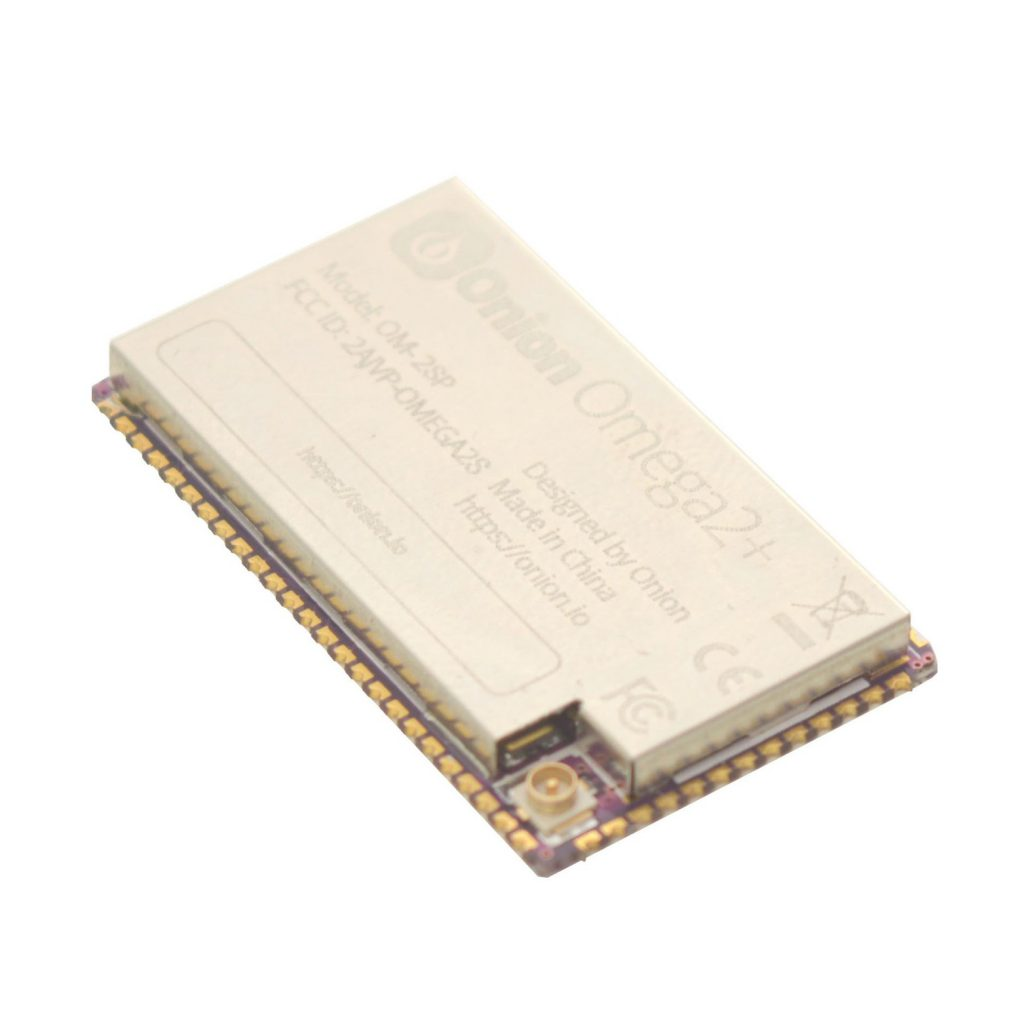
\includegraphics[width=.3\textwidth]{img/Omega2S.jpg}}
    \subfloat[\label{fig:RN4871} RN4871 \cite{microchip_technology_inc_rn4871_nodate}]{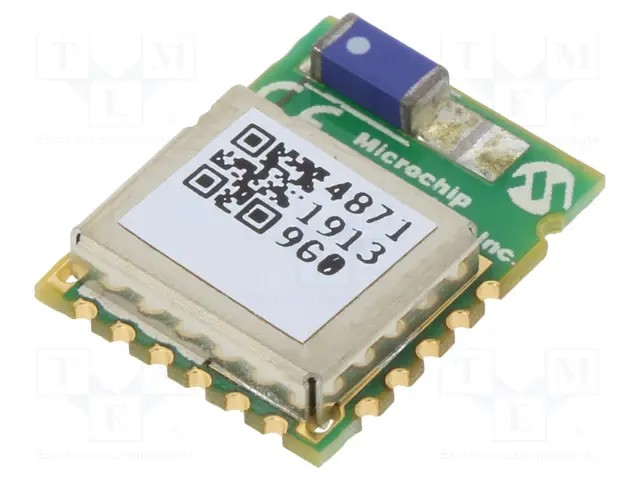
\includegraphics[width=.3\textwidth]{img/rn4871.jpg}}
    \subfloat[MAX F10s \cite{u-blox_max-f10s_2024}]{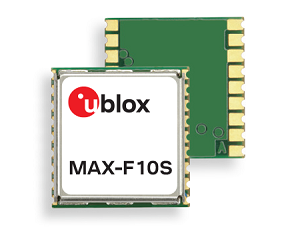
\includegraphics[width=.3\textwidth]{img/max-f10s.png}}
    \caption{\label{fig:wireless-modules} Common wireless modules}
\end{figure}

This approach allows us to separate the usually complex and more expensive multi-layer board layouts, required by modern SOCs, along with their power delivery and any other supporting circuitry, from the less complex end-application consisting of local power regulation, battery management, connectors and other mechanical features.

In order to satisfy the requirements \ref{section:final-requirements}, the module should provide means for analog and digital signal acquisition, digital communication interfaces and sufficient internal storage along with implementing the wireless connectivity.

\subsection{\label{section:mcu}Microcontroller}
Given the requirements for minimal footprint a fully integrated SOC solution is preferred to a configuration of separate MCU and an RF solution. STM32WL series offers such an SOC, which also satisfies the requirement of low power consumption by being based on the STM32L4, a well known ultra low power family of micro-controllers.

The manufacturer also offers a development board, the NUCLEO-WL55JC (\ref{fig:nucleo}), and a plethora of reference designs, the STDES-WL5xxxxx series, where the STDES-WL5U4ILH (\ref{fig:reference-design}) overlaps well with our requirements.

\begin{figure}
    \centering
    \subfloat[\label{fig:nucleo} NUCLEO-WL55JC \cite{stmicroelectronics_nucleo-wl55jc_2024}]{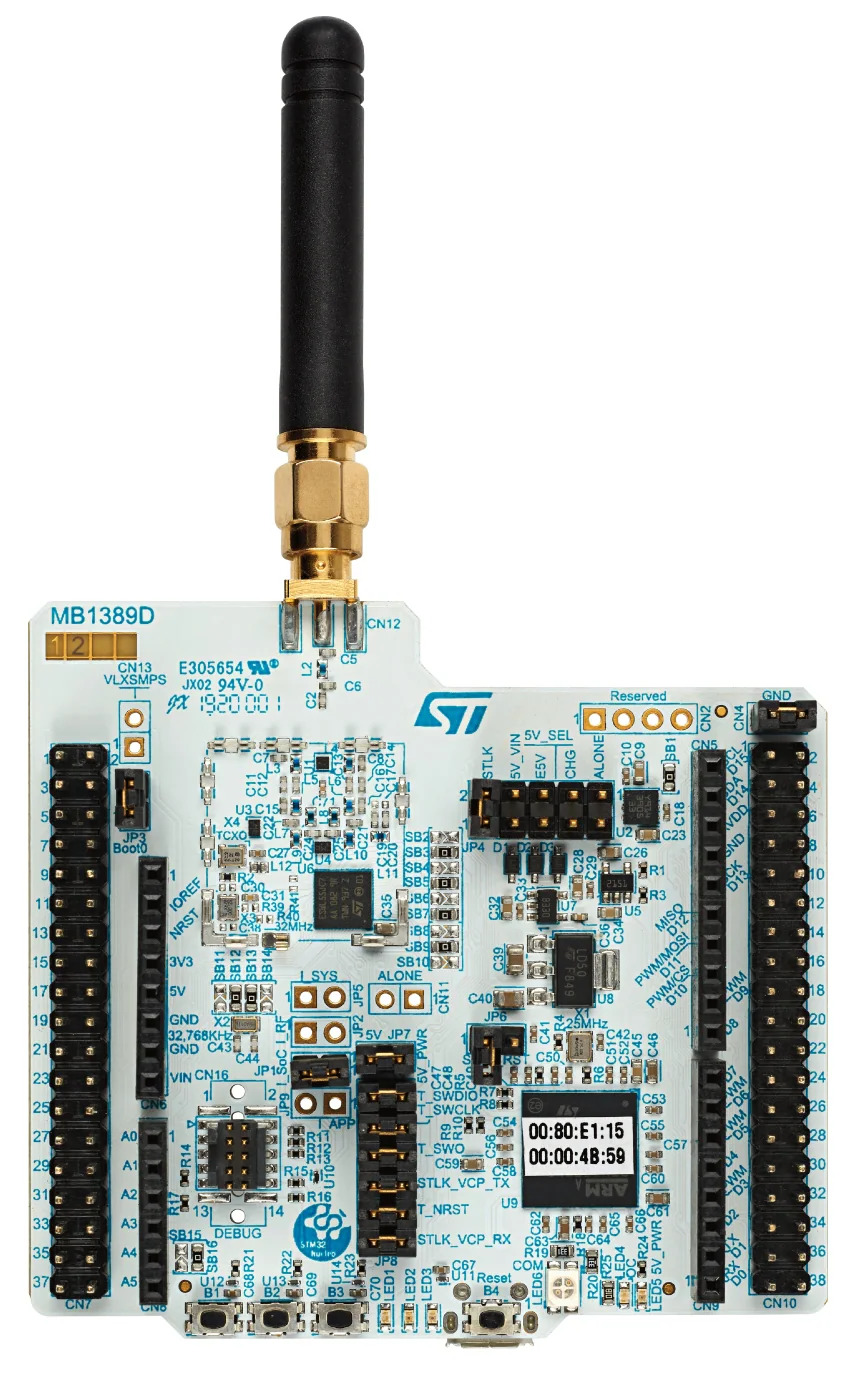
\includegraphics[width=.3\textwidth]{img/nucleo-wl55jc.jpg}}
    \subfloat[\label{fig:reference-design} STDES-WL5U4ILH \cite{stmicroelectronics_stdes-wl5u4ilh_2024}]{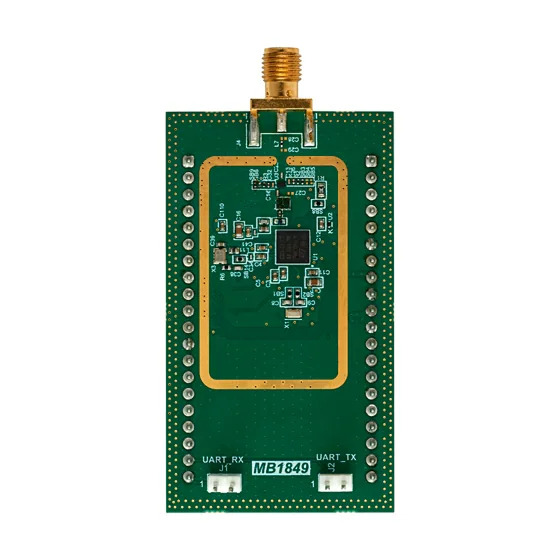
\includegraphics[width=.5\textwidth]{img/STDES-WL5U4ILH.jpg}}
    \caption{\label{fig:nucleo-and-reference} Nucleo development kit and the reference design board}
\end{figure}

Each of the designs focuses on optimizing different parameters depending on the application priorities and their codification follows table \ref{fig:reference-design-codification}, from which the defining features are apparent. For this work, application footprint was one of the top priorities, so the lower-power $15~\mathrm{dB}$ version with IPD was selected.

IPD stands for Integrated Passive Device, it consists of a balun and a harmonic filter. This circuitry is usually realized using passive components, which is cheaper, but takes up more board space (see Figure \ref{fig:frontend-comparison} for comparison), is more prone to design mistakes and tuning mismatch. This particular IPD was specifically designed for STM32WL line of microcontrollers in this configuration \cite{stmicroelectronics_balfhb-wl-05d3_2024}.

\begin{figure}
    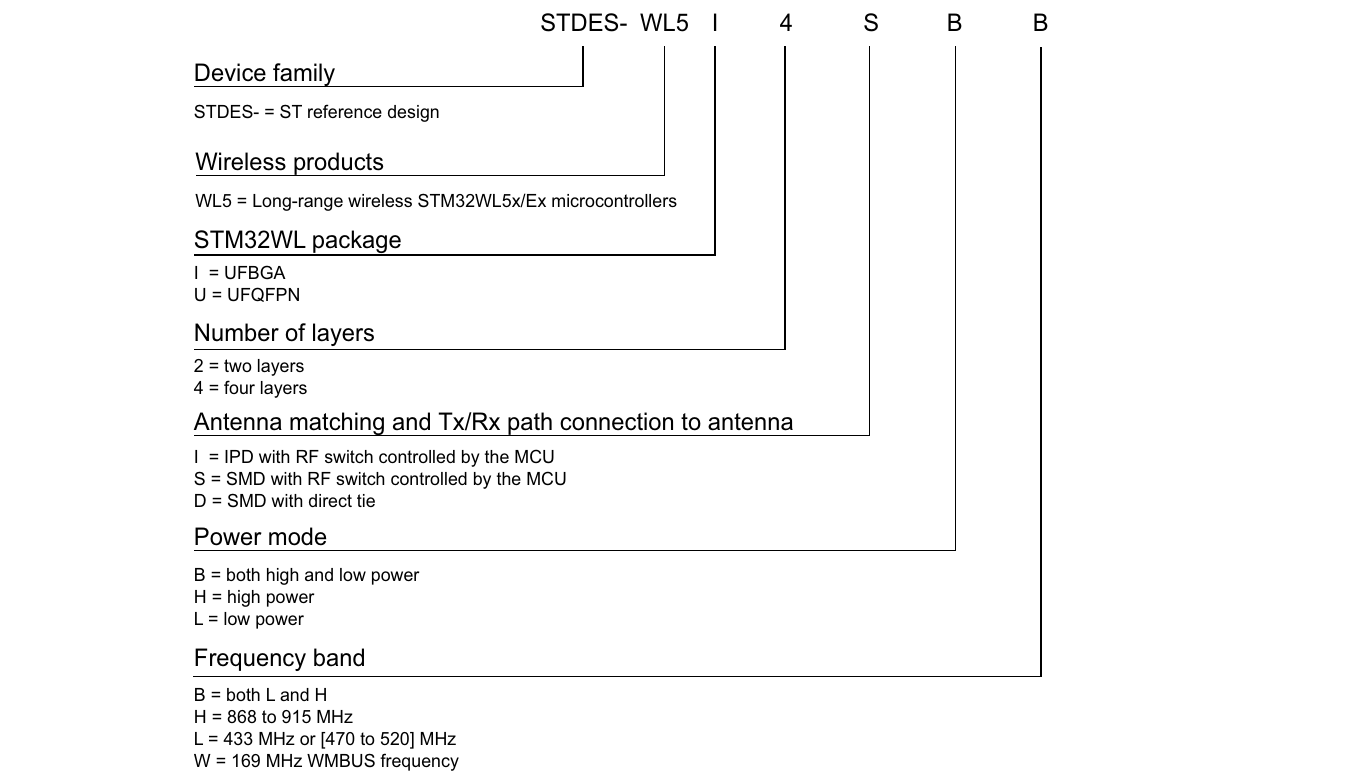
\includegraphics[width=\textwidth]{fig/STDES-xxxxxxx.png}
    \caption{\label{fig:reference-design-codification} STM32WL5x and STM32WLEx reference designs codification}
\end{figure}

\begin{figure}
    \centering
    \subfloat[discrete /wo RF switch (variant D)]{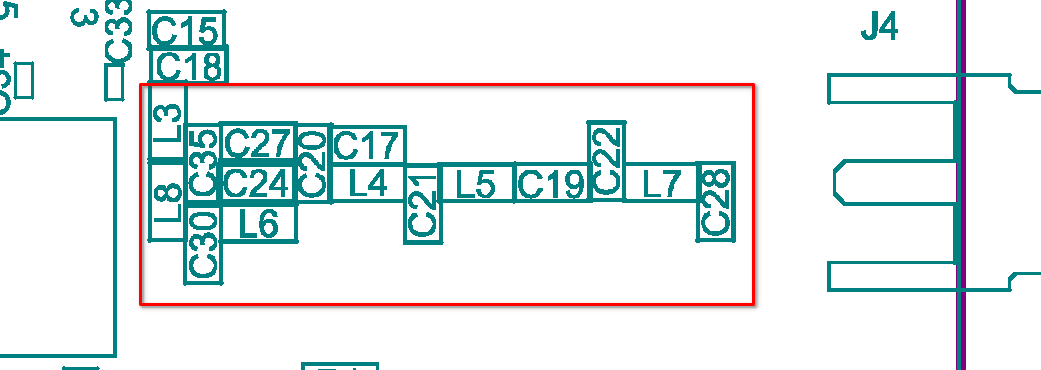
\includegraphics[angle=-90,width=.28\textwidth]{img/frontend-dlb.png}}\hfill
    \subfloat[discrete /w RF switch (variant S)]{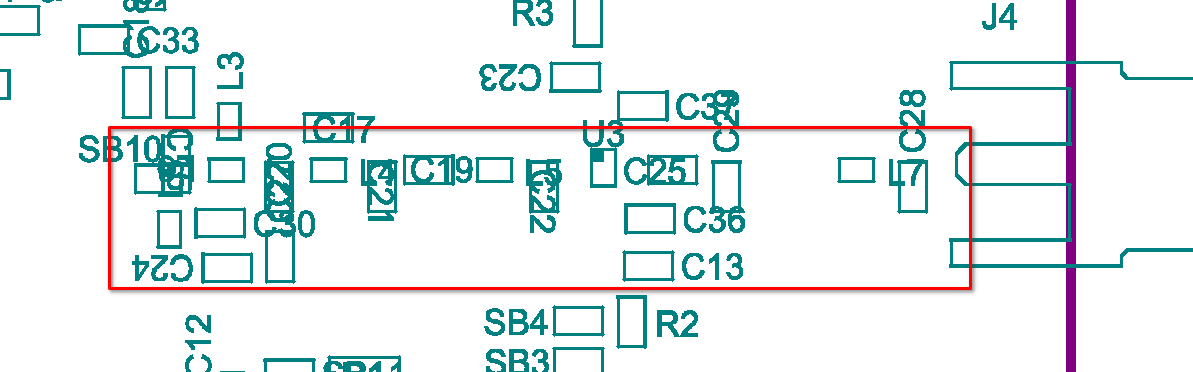
\includegraphics[angle=-90,width=.25\textwidth]{img/frontend-sbb.png}}\hfill
    \subfloat[IPD (variant I)]{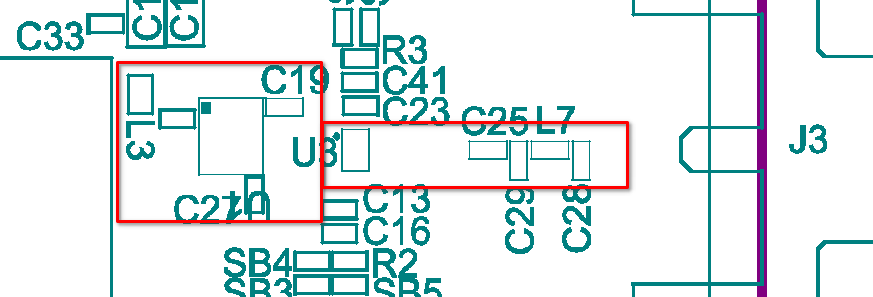
\includegraphics[angle=-90,width=.28\textwidth]{img/frontend-ilh.png}}
    \caption{\label{fig:frontend-comparison} Frontend layout and part selection comparison, components on the RF path highlighted. Reference designs selected for comparison were picked based on the similarity with the STDES-WL5U4ILH design.}
\end{figure}

One downside of using an IPD in this case is that it requires the use of an RF switch, because ST's IPDs are designed to work with separate receive and transmit paths. Again this is a tradeoff between complexity, cost and board space required. Fortunately only a Single Pole Double Throw switch is required, thus a simple switch such as the BGS12SN6 from Infineon \cite{infineon_technologies_bgs12sn6_2024} is sufficient.

A 4 layer reference design was selected because it is anticipated it will allow a higher density layout, shrinking the module dimensions even further. UFQFPN package is preferred over UFBGA to stay compatible with lower cost manufacturing solutions. It is expected the design will use most of the available pins on the package, a complex fanout would be required if we were to go with the BGA variant, perhaps some space savings could be had at the cost of losing access to most of the pins, making any modifications to the design difficult to impossible, should the need arise.

In conclusion, the MCU choice is a culmination of tradeoffs, where the prevention of mistakes, efficiency and familiarity were more important than the absolute performance and cost. This should not in any way hamper further improvements in succeeding versions of this hardware, while allowing the completion of Proof-of-Concept stages of this project. 

\subsection{Power}
The selected MCU supports wide input voltage of $2-3.6~\mathrm{V}$ thanks to its internal voltage regulation. It supports two modes - LDO, which does not require any additional external component at the cost of lower efficiency and the SMPS mode, utilizing a synchronous buck regulator, which is more efficient - this application will therefor attempt to implement the latter.

A separate, switchable power-rail is a feature deemed necessary by some considered applications in \ref{section:application-case-studies}. This can be achieved using a built-in MOSFET - such power rail could be used to save power even by powering off some parts of the module itself.

\subsection{Non-volatile memory}

\subsection{Antenna}
In the initial module requirements \ref{section:final-requirements} it was deemed preferable to integrate the antenna onto the module itself. This should not, however, compromise on the usability and performance of the module. 

In general, there are two approaches for integrated antennae - a trace antenna constructed using the PCB directly, or an antenna in the form of a solderable component, such as an ceramic chip antenna. If the board space is limited, the performance is insufficient or the use of an integrated antenna is prohibited by any other limitation, the application must resort to an external antenna connected to the RF circuitry through a coaxial cable. The table \ref{table:antenna-solutions} provides a good summary.

\begin{table}[H]
\begin{center}
\caption{\label{table:antenna-solutions}Advantages and Disadvantages of different antenna solutions \cite{andersen_selecting_2008}}
    \begin{tabular}{|l|l|l|}
    \hline
    \textbf{Antenna types} & \textbf{Advantages} & \textbf{Disadvantages} \\
    \hline
    PCB antenna  & Low cost, No assembly,        & Difficult to design small \\
                 & Good performance achievable,  & and efficient antenna, \\
                 & Small size at high frequency  & Large size at low frequency \\
    \hline
    Chip antenna & Small size,                   & Medium performance, \\
                 & Off-the-shelf solution        & Medium cost \\
    \hline
    Whip antenna & Good performance,             & High cost, \\
                 & Off-the-shelf solution        & Large size \\
    \hline
    \end{tabular}
\end{center}
\end{table}

The following sections elaborate on each antenna type in more detail in the context of this particular application. 

At this point in the design process, the module proportions, derived from the individual component footprints, are not expected to surpass $500~\mathrm{mm^2}$. It is also expected the design will need to conform to the PCB parameters specified in Table \ref{table:pcb-parameters}. Since the first prototypes will only operate in Europe, the aim is mainly the EU868 band.

\begin{table}[H]
\begin{center}
\caption{\label{table:pcb-parameters}Approximate PCBWay manufacturer stackup parameters \cite{pcbway_stackup_2024}}
    \begin{tabular}{|l|l|} \hline
    \textbf{Parameter}            & \textbf{Value} \\ \hline
    Stackup thickness             & $1.6~\mathrm{mm}$ \\ \hline
    Substrate dielectric constant & $4.5~\mathrm{[-]}$ \\ \hline
    Substrate loss tangent        & $0.02~\mathrm{[-]}$ \\ \hline
    \end{tabular}
\end{center}
\end{table}

\subsubsection{Printed Circuit Board antenna}
Due to the limited board space, this option is expected to not be feasible. Nevertheless, some types of PCB antenna solutions were calculated to support this intuition.

A microstrip patch antenna is one of the simplest types of PCB antenna designs \cite{zachariah_peterson_microstrip_2022,wallace_an058_nodate}. This antenna consists of the patch itself and its feed-line with optional inset for impedance matching, see \ref{fig:patch-antenna}. 

The approximate parameters presented in Table \ref{table:antenna-pcb-calculations} were obtained using \cite{zachariah_peterson_microstrip_2022}, the input impedance could be tuned using the inset and a matching circuit, but more importantly, this simple antenna design is not practical because of its size, which already has roughly 15 times the surface area of the module components.

Another, more space-efficient option, is to use the inverted-F design, see Figure \ref{fig:inverted-f-antenna} for its simplest form. We can calculate its length $L$ given the target frequency $f$
\begin{equation}
    % 299,792,458/(4*868,000,000)
    L = \dfrac{\lambda}{4} = \dfrac{c_0}{4f} = \dfrac{c_0}{4 \cdot 868 \cdot 10^6} \approx 86.3~\mathrm{mm}
\end{equation}
which is a great improvement compared to the patch antenna.

This design could perhaps be optimized such that it would fit the size constraints, but such work might be enough to write another thesis focused on just this detail. Dimensions based on the layout in Figure \ref{fig:inverted-f-antenna} were included in Table \ref{table:antenna-pcb-calculations} for comparison sake.

\begin{figure}
    \centering
    \subfloat[\label{fig:patch-antenna}Microstrip patch antenna dimensions including the feed-line \cite{zachariah_peterson_microstrip_2022}]{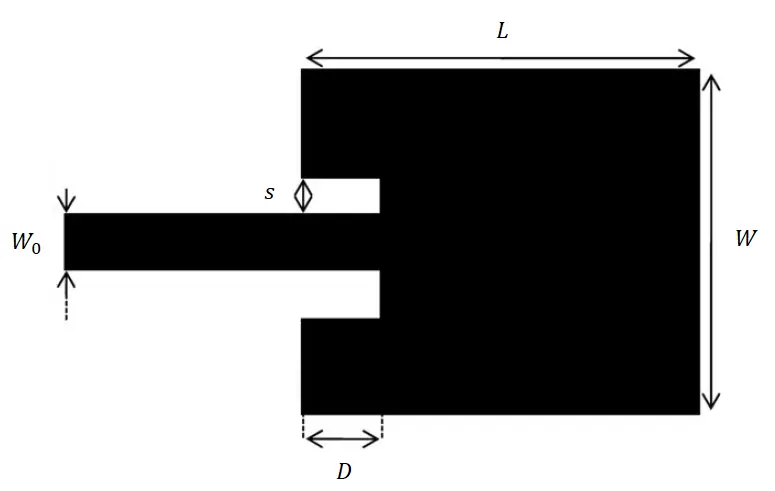
\includegraphics[width=.53\textwidth]{fig/patch-antenna.png}}\hfill
    \subfloat[\label{fig:inverted-f-antenna}Basic inverted-F antenna design \cite{peterson_inverted-f_2023}]{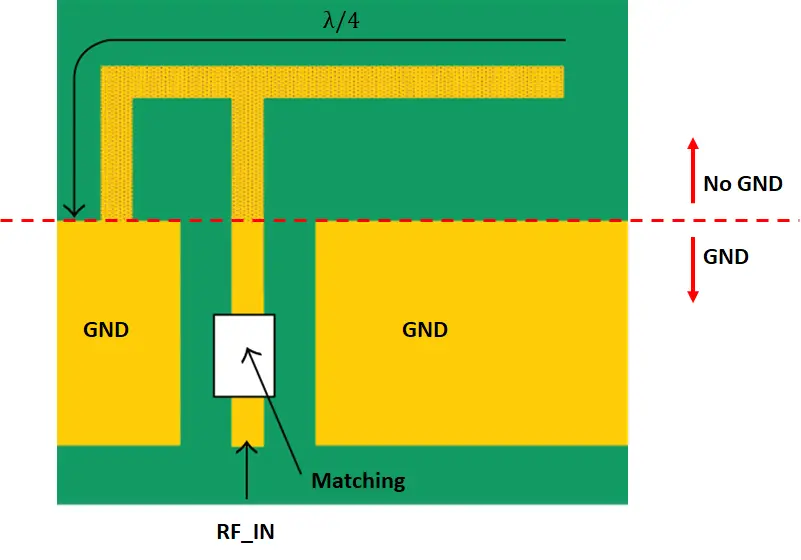
\includegraphics[width=.43\textwidth]{fig/inverted-f-antenna.png}}
    \caption{Simple Printed Circuit Board antenna designs}
\end{figure}

\begin{table}[H]
\begin{center}
\caption{\label{table:antenna-pcb-calculations}Approximate microstrip patch antenna parameters and dimensions (as described in \ref{fig:patch-antenna}) and a notion of the dimensions of an inverted-F antenna (corresponding to \ref{fig:inverted-f-antenna}), not including the ground-plane and matching network}
    \begin{tabular}{|l|l|l|} \hline
    \textbf{Parameter}  & \textbf{Patch antenna}    & \textbf{Inverted-F antenna} \\ \hline
    Input impedance     & $306~\mathrm{\Omega}$     & not calculated \\ \hline
    Bandwidth           & $3.92~\mathrm{MHz}$       & not calculated \\ \hline
    Width (W)           & $104~\mathrm{mm}$         & $\approx 70~\mathrm{mm}$ \\ \hline
    Length (L)          & $80~\mathrm{mm}$          & $\approx 18~\mathrm{mm}$ \\ \hline
    Minimum footprint   & $8320~\mathrm{mm^2}$      & $1260~\mathrm{mm^2}$ \\ \hline
    \end{tabular}
\end{center}
\end{table}

These preliminary calculations led to the conclusion, that a PCB antenna at this frequency with these size constraints is not viable in this case. These calculations are not even beginning to factor in all the other components required, not to mention the even larger ground-plane which such antenna would require. 

This could be made possible with significant design effort and expertise, or by licensing an existing design, but the overall goal of creating this hardware would need to shift as a result.

\subsubsection{Chip antenna}
As outlined in \ref{table:antenna-solutions}, the chip antenna is another logical step in the search of the right solution. It is a common choice seen in commercially available hardware, especially in cases, where the space is at a premium - as can be seen on the RN4871 \ref{fig:RN4871} Bluetooth module.

There is a large selection of these antennae on the market, mainly targeted at the very common bands, such as $2.4~\mathrm{GHz}$ and $5~\mathrm{GHz}$, but solutions for the $868~\mathrm{MHz}$ frequency range are also not hard to come by \cite{digikey_rf_2024,mouser_europe_868_2024}.



\subsection{Conclusion}
We managed to meet all requirements set in \ref{section:final-requirements} except

\FloatBarrier
\section{Sensor architecture}
Given the aim of this project

\subsection{Expected capacitance range}

\subsection{Measuring method}

\subsection{Battery and charging}

\chapter{\label{chapter:results}Results}
%!TEX ROOT=main.tex

\section{LoRa Module Design}
As discussed in section \ref{section:module-architecture}, where the LoRa module was architected and its main parts were selected, the schematic and board layout were created. These outputs are included in image form as Appendix \ref{chapter:module01-files}, along with more details, and available at \link{https://github.com/manakjiri/lora-module-hw/releases/tag/v0.1}{github.com/manakjiri/lora-module-hw}.

The Open source KiCad Electronic Design Automation (EDA) software was used throughout the project to create these designs.

\subsection{\label{section:module-schematic}Schematic}
While the \ref{section:module-architecture} focused on the fundamental parts of the design, many details were left up to the later development stages, once the overall system implementation is more clear. This section will focus and expand on these parts of the design.

Of note is the selection of the main clock source for the MCU \ref{section:mcu}. In this case the only two options are to use a Crystal oscillator (XO) or an Temperature Compensated XO (TCXO). Application note AN5646 (STMicroelectronics \cite{stmicroelectronics_how_nodate-1}) summarizes the main differences as
\begin{itemize}
    \item An XO is more efficient on power consumption, startup time, and BOM cost.
    \item A TCXO is more efficient on frequency accuracy and frequency variation over temperature changes. It also
    removes layout constraints.
\end{itemize}

This aspect was not considered carefully enough during the parts selection, the recommended NX2016SA series crystal oscillator was selected for the power savings and reduced cost. However, the selected programming framework, Embassy, and the library lora--rs in particular (expanded upon in Appendix \ref{chapter:rust}), only correctly supported the use of an TCXO, at the time of the prototype bring--up. This led to an ad hoc modification, documented in Figure \ref{fig:tcxo-bodge}, of the module and the addition of the Abracon ATX--11--F series TCXO to fix this issue.

\begin{figure}
    \centering
    \subfloat[top view]{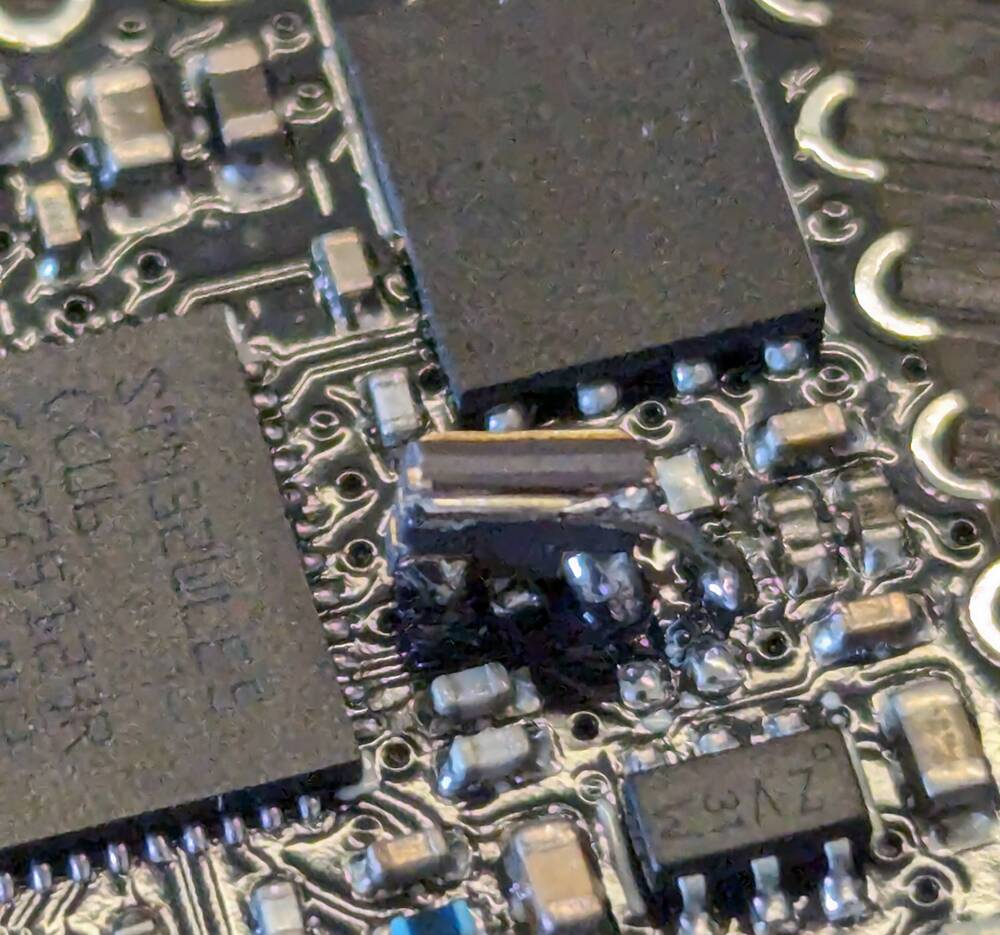
\includegraphics[width=.30\textwidth]{img/tcxo-bodge1.jpg}} \hfil
    \subfloat[side view]{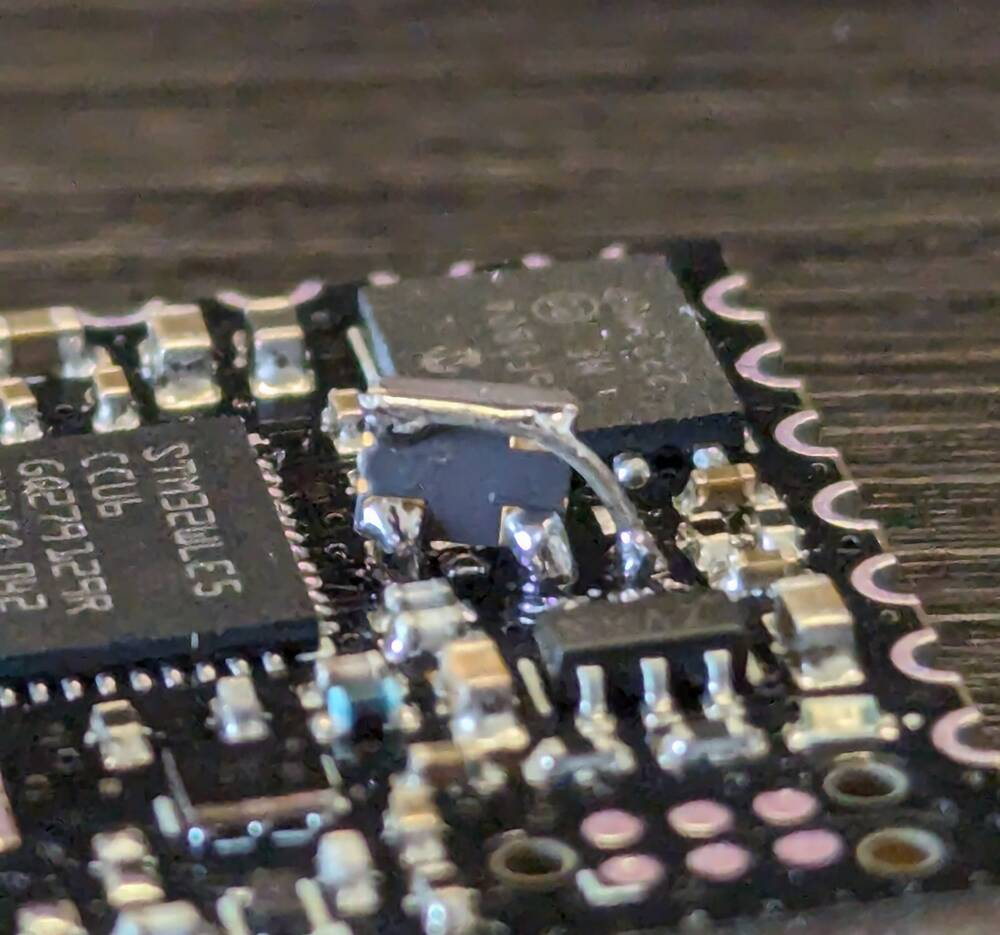
\includegraphics[width=.30\textwidth]{img/tcxo-bodge2.jpg}}
    \caption{\label{fig:tcxo-bodge}The ad hoc TCXO modification on the LoRa module.}
\end{figure}

All other aspects of the MCU integration were executed according to the application notes and the datasheet  \cite{stmicroelectronics_stm32wle5xx_nodate,stmicroelectronics_how_nodate-1}, while closely following the implementations of the reference design and the nucleo development kit \cite{stmicroelectronics_stdes-wl5u4ilh_2024,stmicroelectronics_nucleo-wl55jc_2024}. This includes the selection of decoupling capacitors, the SMPS circuitry and the reset handling.

Another consideration was the implementation of the switchable power rail VDD\_SW. This rail taps off the main power rail of the rest of the module, any disruption could cause a glitch or trigger the BOR protection circuitry. It is thus necessary to limit the inrush current caused by this rail's switch--on and subsequent charging of any local capacitances. An RC circuit was designed to slow--down the gate voltage rise--time to about 10 ms.

\subsection{Printed Circuit Board Layout}
A 4 layer board stackup was proposed in Section \ref{section:mcu}, which indeed ended up being used in this design. Purpose of each layer is described in table \ref{table:board-layers} and clearly observable in the final renders \ref{board:v0.1}.

\begin{table}[H]
\begin{center}
\caption{\label{table:board-layers}Module board layer signal and power assignments.}
    \begin{tabular}{|l|l|} \hline
    \textbf{Layer name}     & \textbf{Primary purpose} \\ \hline
    F. Front layer          & Components and local connections \\ \hline
    1. First inner layer    & Ground \\ \hline
    2. Second inner layer   & Power \\ \hline
    B. Back layer           & Signal and markings \\ \hline
    \end{tabular}
\end{center}
\end{table}

The board is only populated on the front side, see Figure \ref{board:v0.1-components}, to allow its use as a solder--able module. Still, the final dimensions of the module are $20.32 \times 22.48~\mathrm{mm}$, which is better than the initial optimistic estimate given in Section \ref{section:antenna}.

To stay compatible with low--cost manufacturing options, conservative parameters were picked when it comes to minimal clearance, trace width and drill size. No density--increasing technologies, such as blind or buried vias, via--in--pad, micro--via, etc. were employed either. 

These parameters are summarized in the following Table \ref{table:board-limits} and were enforced by the Design Rule Checker (DRC) throughout the project.

\begin{table}[H]
\begin{center}
\caption{\label{table:board-limits}Board layout physical limits.}
    \begin{tabular}{|l|l|} \hline
    \textbf{Parameter}          & \textbf{Dimension} \\ \hline
    Minimum trace clearance & $0.15~\mathrm{mm}$ \\ \hline
    Minimum trace width & $0.15~\mathrm{mm}$ \\ \hline
    Minimum via width & $0.3~\mathrm{mm}$ \\ \hline
    Hole to trace clearance & $0.3~\mathrm{mm}$ \\ \hline
    Hole to hole clearance & $0.5~\mathrm{mm}$ \\ \hline
    Board edge to trace clearance & $0.15~\mathrm{mm}$ \\ \hline
    \end{tabular}
\end{center}
\end{table}

Being only 4 layers, the traces needed to be routed in densely and well thought--out manner, attempting to minimize the number of relatively large vias required. For this reason, the module's external connection signal assignments were decided only near the end of the design stage conforming mostly to the existing pin locations on the MCU itself. The final pad assignments are included in Table \ref{table:module-pin-legend}.

\begin{figure}
    \includesvg[width=.75\textwidth]{img/module-v0.1.drawio.svg}
    \caption{\label{fig:module-v0.1}Image of the manufactured and fully assembled module with overlay highlighting its functional parts.}
\end{figure}

\subsection{Finalized LoRa Module Specification}
Figure \ref{fig:module-v0.1} shows the manufactured and fully assembled module with overlay highlighting its functional parts, its technical specifications are captured by Table \ref{table:module-specification}.

\begin{table}[p]
\begin{center}
\caption{\label{table:module-specification}Final module specification.}
    \begin{tabular}{|l|l|} \hline
    Supply voltage range                    & $2.3\text{--}3.5~\mathrm{V}$\\ \hline
    Maximum supply current (excluding EXT)  & $65~\mathrm{mA}$\\ \hline
    %Standby supply current                  & $10--500~\mathrm{uA}$\\ \hline
    Operating temperature range             & $-40\text{--}85~\mathrm{^\circ C}$\\ \hline
    Output RF power                         & $15~\mathrm{dBm}$\\ \hline
    Operating band                          & $868~\mathrm{MHz}$\\ \hline
    RF connector                            & U.FL \\ \hline
    Module connection type                  & Castellated hole (0.1 inch pitch) \\ \hline
    Supported interfaces                    & UART, SPI, I2C \\ \hline
    Programming interface                   & ARM Serial Wire Debug (SWD) \\ \hline
    \end{tabular}
\end{center}
\end{table}

\begin{table}[p]
\begin{center}
\caption{\label{table:module-pin-legend}Module pin legend including feature summary.}
    \begin{tabular}{|l|l|l|l|l|l|l|l|l|} \hline
    \textbf{IO} & \textbf{Pin} & \textbf{TIM\footnote{Refer to each column following ``Pin'' (excluding ``Other'') as [Column header][Column-row contents], such as ``SPI1\_MOSI'' and so on. Some features were omitted for clarity, for complete list refer to the MCU manufacturer's documentation}} & \textbf{ADC} & \textbf{I2C} & \textbf{SPI} & \textbf{UART} & \textbf{Other}\\ \hline
    1  & PA7  & 17\_1, 1\_1N    &     & 3\_SCL & 1\_MOSI &             & CMP2\_OUT          \\ \hline
    2  & PA6  & 16\_1          &     &       & 1\_MISO &             &                    \\ \hline
    3  & PA4  & L1,2\_OUT      &     &       &        &             & RTC\_OUT2           \\ \hline
    4  & PA2  & 2\_3           &     &       &        & 2\_TX      & CMP2\_OUT           \\ \hline
    5  & PA1  & L3\_OUT, 2\_2   &     &       & 1\_SCK  &             &                    \\ \hline
    6  & PA0  & 2\_1           &     &       &        &             & WKUP1   \\ \hline
    7  & PB8  & 16\_1, 1\_2N    &     & 1\_SCL &        &             &                    \\ \hline
    8  & PB7  & L1\_IN2, 17\_1N &     & 1\_SDA &        & 1\_RX        &                    \\ \hline
    9  & PB6  &               &     & 1\_SCL &        & 1\_TX        &                    \\ \hline
    10 & PB5  & L1\_IN1        &     &       & 1\_MOSI &             & CMP2\_OUT          \\ \hline
    11 & PB4  &               & 3   & 3\_SDA & 1\_MISO &             & CMP1,2\_INP        \\ \hline
    12 & PA11 & 1\_4           & 7   & 2\_SDA & 1\_MISO &             & CMP1,2\_INM        \\ \hline
    13 & PB3  & 2\_CH2         & 2   &       & 1\_SCK  &             & SWO, WKUP3 \\ \hline
    14 & PA13 &               & 9   &       &        &             & SWDIO            \\ \hline
    15 & PA14 & L1\_OUT        & 10  &       &        &             & SWCLK                   \\ \hline
    16 & PH3  &               &     &       &        &             & BOOT0                   \\ \hline
    \end{tabular}
\end{center}
\end{table}

\subsection{Radio Performance}
The output RF characteristics were validated using a spectrum analyzer connected directly to the RF output of the module through an U.FL pigtail.

The module was setup in ``continuous wave'' mode \cite{semtech_corporation_sx12612_2024} at 869.525 MHz with power of 15 dBm, which produced the spectrogram visible in Figure \ref{fig:rf-mask-wave}. Here we can observe, that the peak power was measured at 12.60 dBm and the frequency is off by 150 kHz.

\begin{figure}
    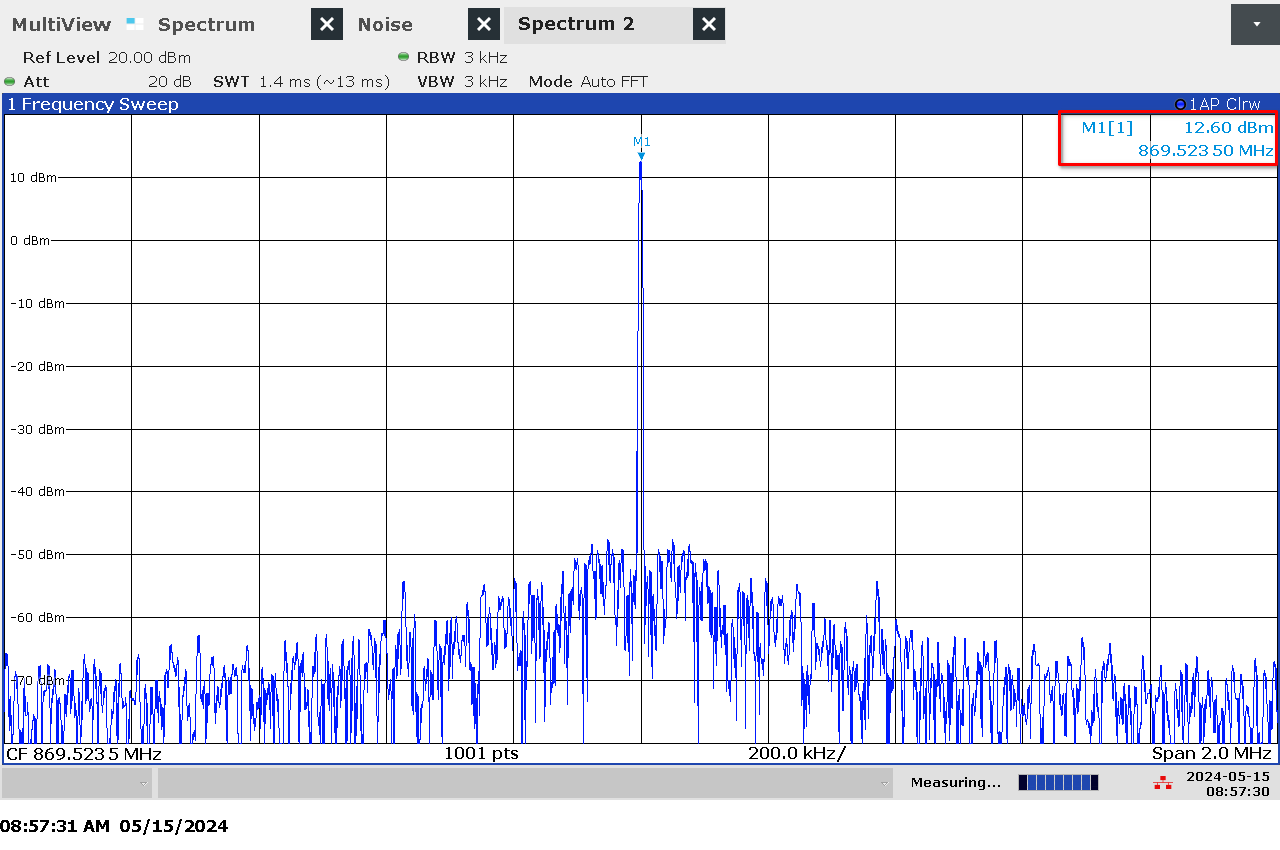
\includegraphics[width=.9\textwidth]{fig/rf-mask-wave.png}
    \caption{\label{fig:rf-mask-wave}Measurement of the module RF output in ``continuous wave'' mode at 869.525 MHz with power of 15 dBm}
\end{figure}

Next two measurements in Figure \ref{fig:rf-power}, are captures of the module transmitting 8 bytes of data at SF5, bandwidth 250 kHz and coding rate 4:5, the rest of the parameters is identical as in Table \ref{table:range-test-parameters}. 

These measurements show that the output power stays stable at 13 dBm once modulating and that there are smooth transitions and power ramp up, suggesting good power supply and power management design. The mask visible in the spectrum is uniform, without any unexpected artifacts.

\begin{figure}[p]
    \centering
    \subfloat[Spectogram of the transmitted signal (upper), waterfall graph of the spectrum (lower)]{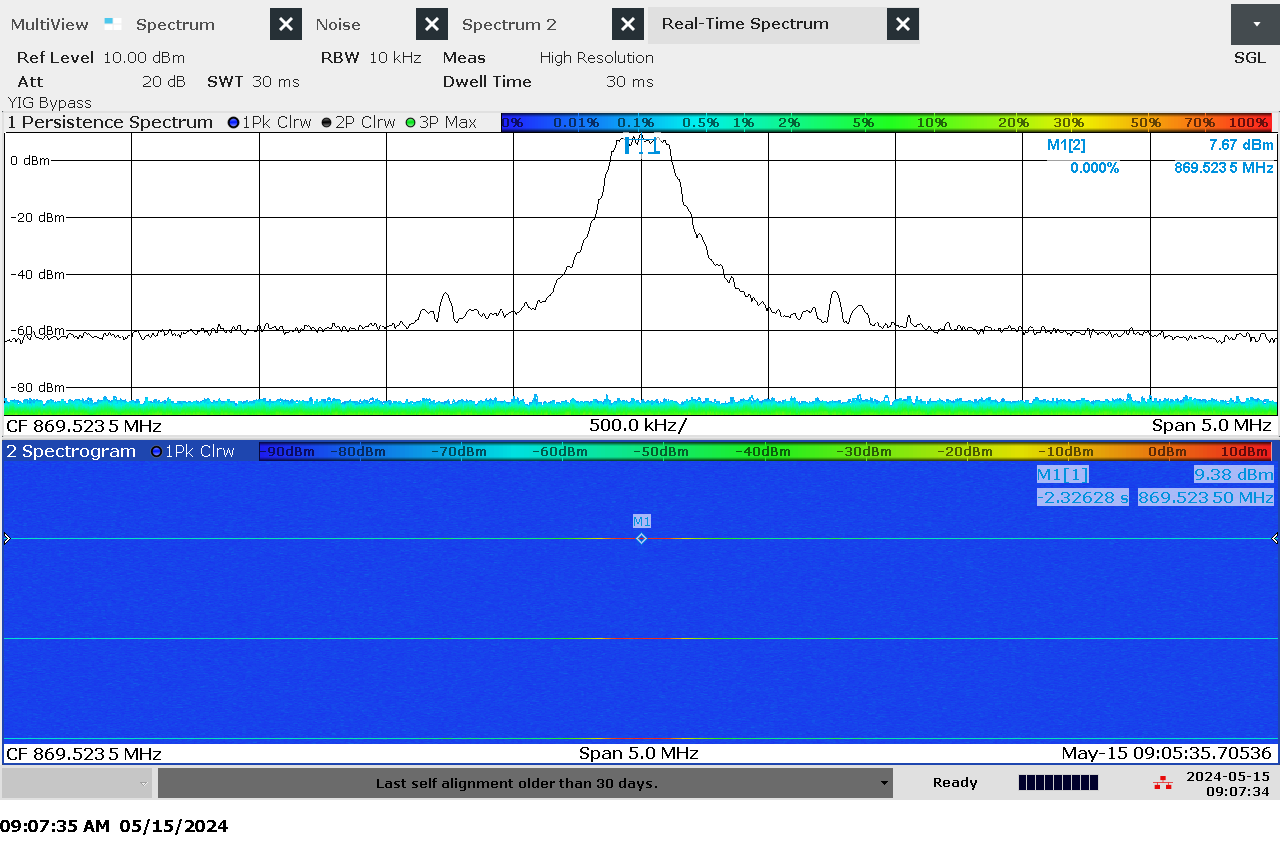
\includegraphics[width=.9\textwidth]{fig/rf-transmit-250khz.png}} \hfil
    \subfloat[Packet in the time domain (upper), Packet spectrum (lower)]{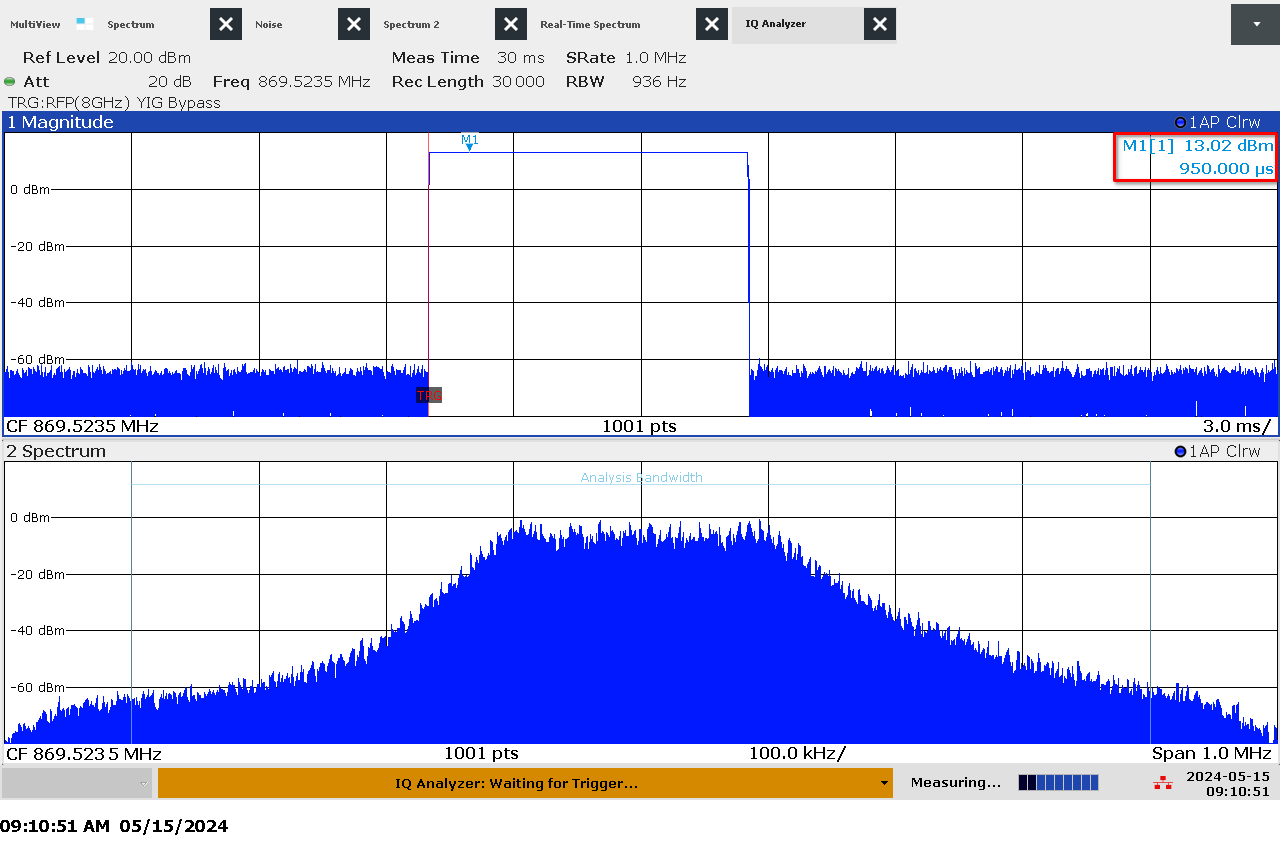
\includegraphics[width=.9\textwidth]{fig/rf-power.png}}
    \caption{\label{fig:rf-power}Capture of the module transmitting 8 bytes of data at SF5, bandwidth 250 kHz and coding rate 4:5, the rest of the parameters is identical as in Table \ref{table:range-test-parameters}}
\end{figure}

\subsection{Power Consumption}
Because of the improvised replacement of the crystal oscillator with a TCXO, which exhibits much higher power consumption (2--3 mA) and an inability to connect its power supply to the pin PB0, which is designed to power this oscillator and gate its power supply whenever it is not needed, the module exhibits higher than expected power draw of around 9 mA while receiving and 6 mA while idle. The fix is documented in Section \ref{section:module-v0.2}.

\begin{figure}
    \centering
    \subfloat[Continuous receive with transmit in the middle]{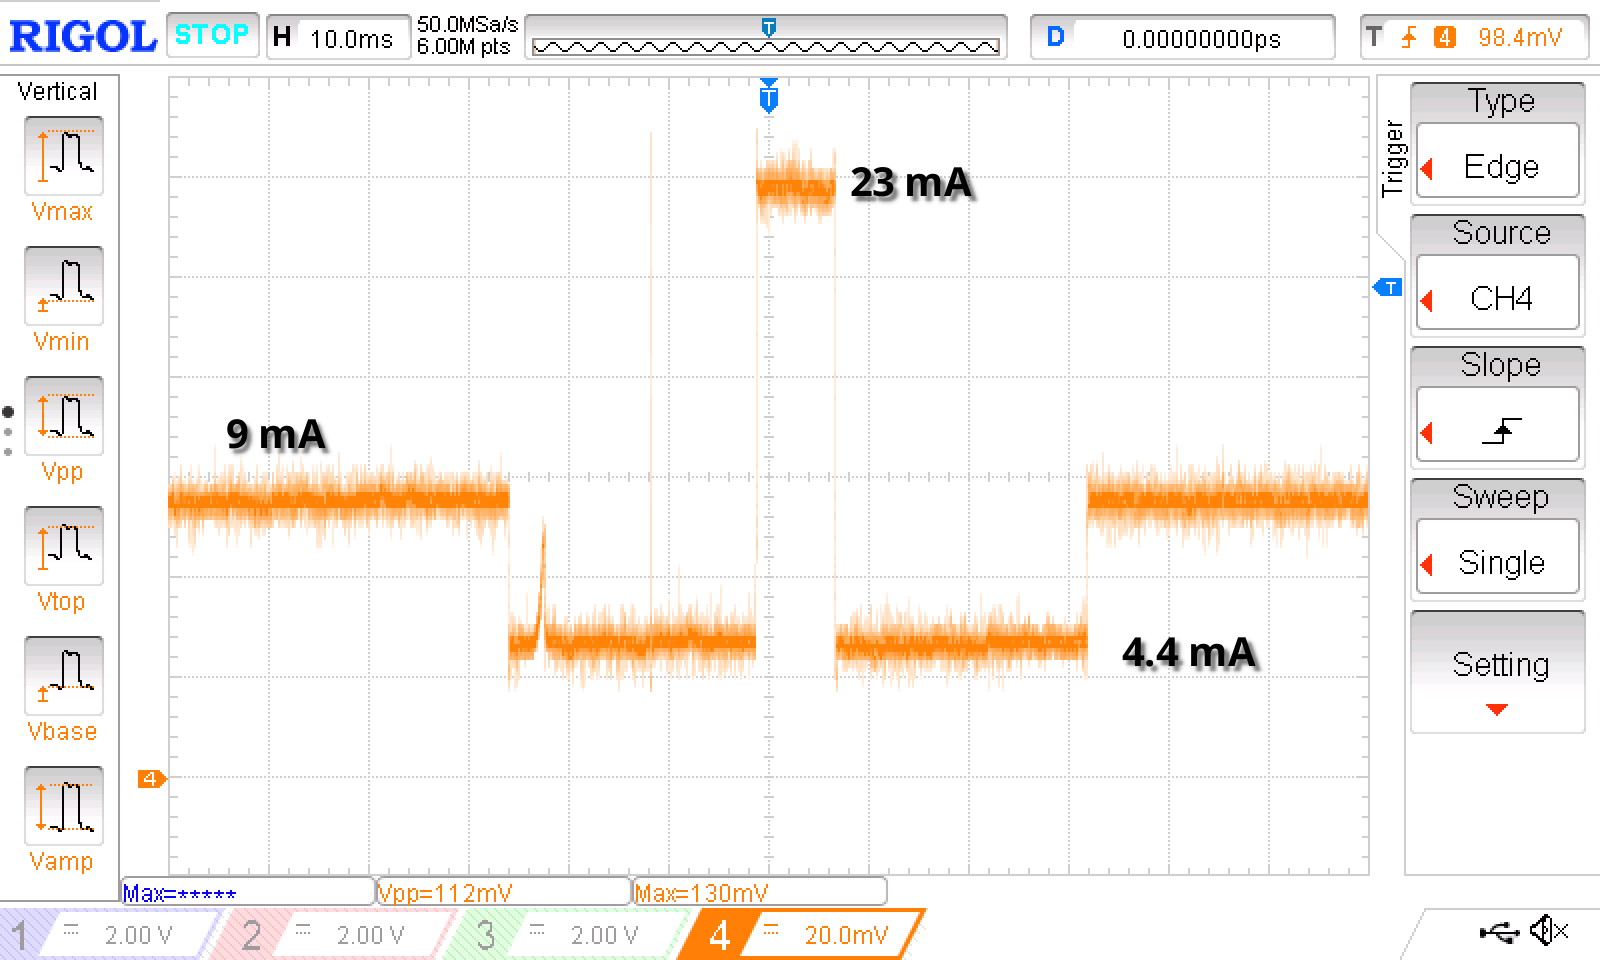
\includegraphics[width=.49\textwidth]{fig/module-current-rx-inv.png}} \hfil
    \subfloat[Idle, transmit, receive acknowledge]{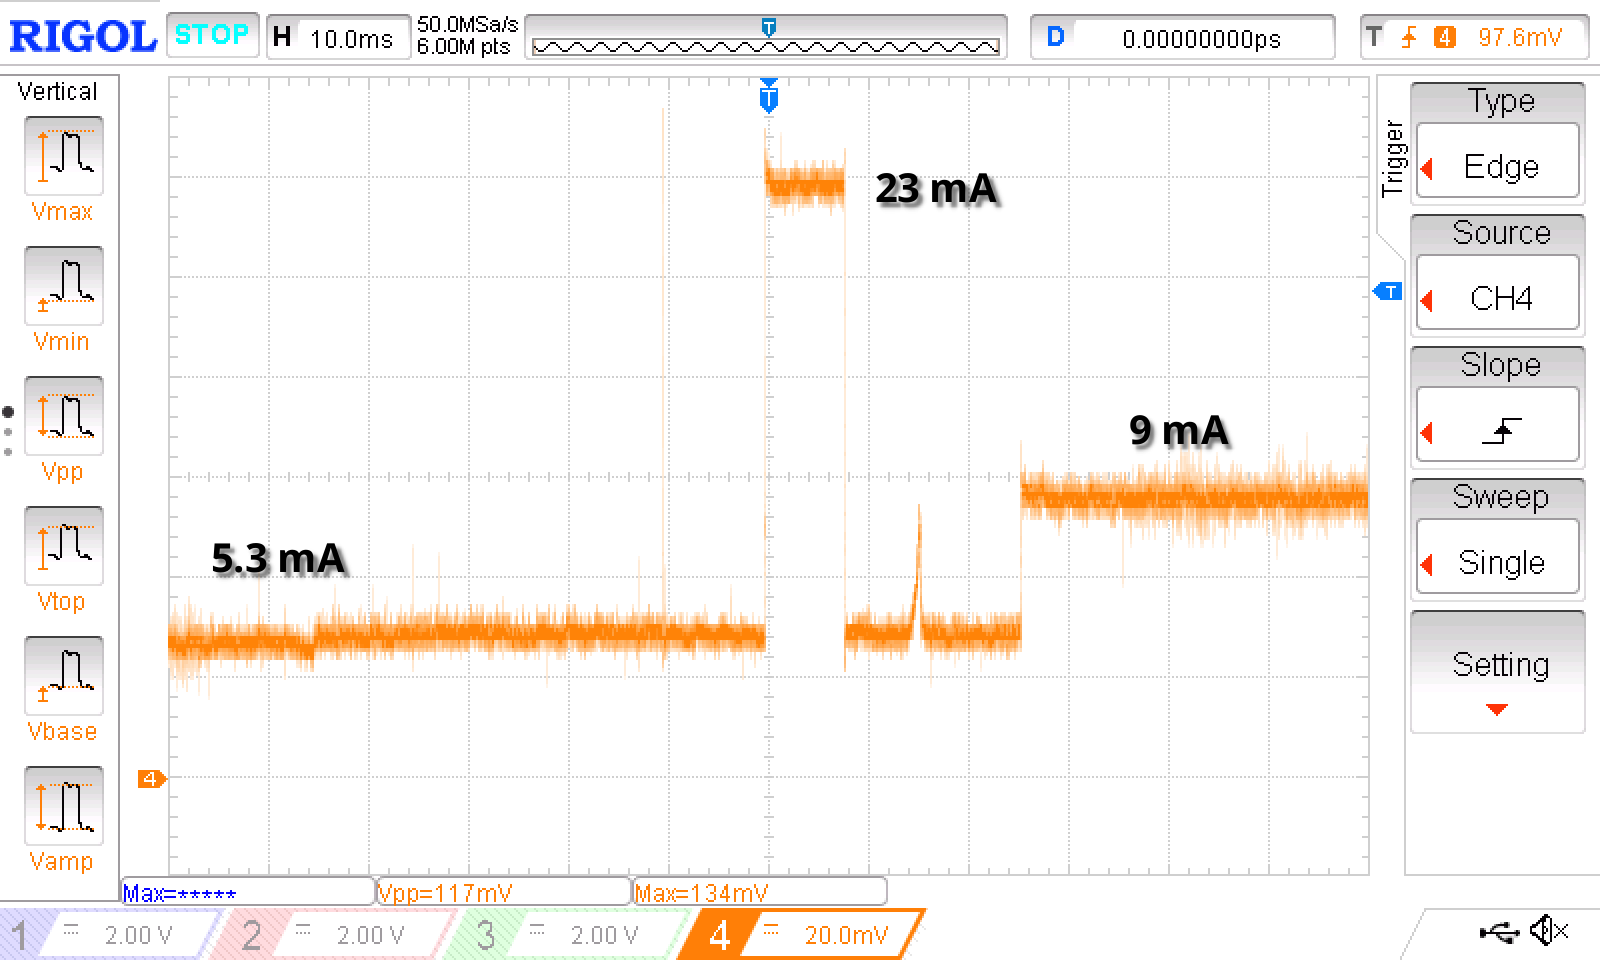
\includegraphics[width=.49\textwidth]{fig/module-current-tx-inv.png}}
    \caption{\label{fig:module-current}Current waveform of the module measured through a 5.6 $\Omega$ resistor in different operational scenarios.}
\end{figure}

The idle power draw could be optimized to reach 10--100s of $\mu$A with the TCXO properly connected and significant time investment into the firmware development. The current consumption waveform can be examined in Figure \ref{fig:module-current}.

\section{Soil Moisture Sensor Design}
\begin{figure}[H]
    \includesvg[width=\textwidth]{boards/sensor/soil-sensor-F_Cu.svg}
    \caption{\label{fig:sensor-pcb}Printed Circuit Board design of the top layer of the soil moisture sensor board, where the 4 capacitive sensing zones are distinctly visible. These capacitors form, what is later referred to, as the ``active area'' of the sensor. More is available in Appendix \ref{chapter:sensor-files}.}
\end{figure}
To summarize, the soil moisture sensor board contains
\begin{itemize}
    \item the capacitance measuring circuit (as described in Section \ref{section:measuring-method}) with two ranges,
    \item a dual single pole quadruple throw (Dual SP4T) mux chip for switching between the 4 sensing zones contained in the active area of the sensor,
    \item 8 channel TVS diode array to clamp the voltage on the capacitor electrodes and means of isolating the sensor elements from the measuring circuits,
    \item a 2.8 V linear low-dropout (LDO) regulator,
    \item footprint for the LoRa module,
    \item two analog temperature sensor ICs and
    \item single cell rechargeable lithium battery protection circuitry.
\end{itemize}

\subsection{\label{section:sensor-circuit}Capacitance Measuring Circuit}
Of note is the performance of the capacitance measuring circuit, which was validated using an oscilloscope connected to the test-points on the sensor board, see Figure \ref{fig:cap-measure}.
\begin{figure}[H]
    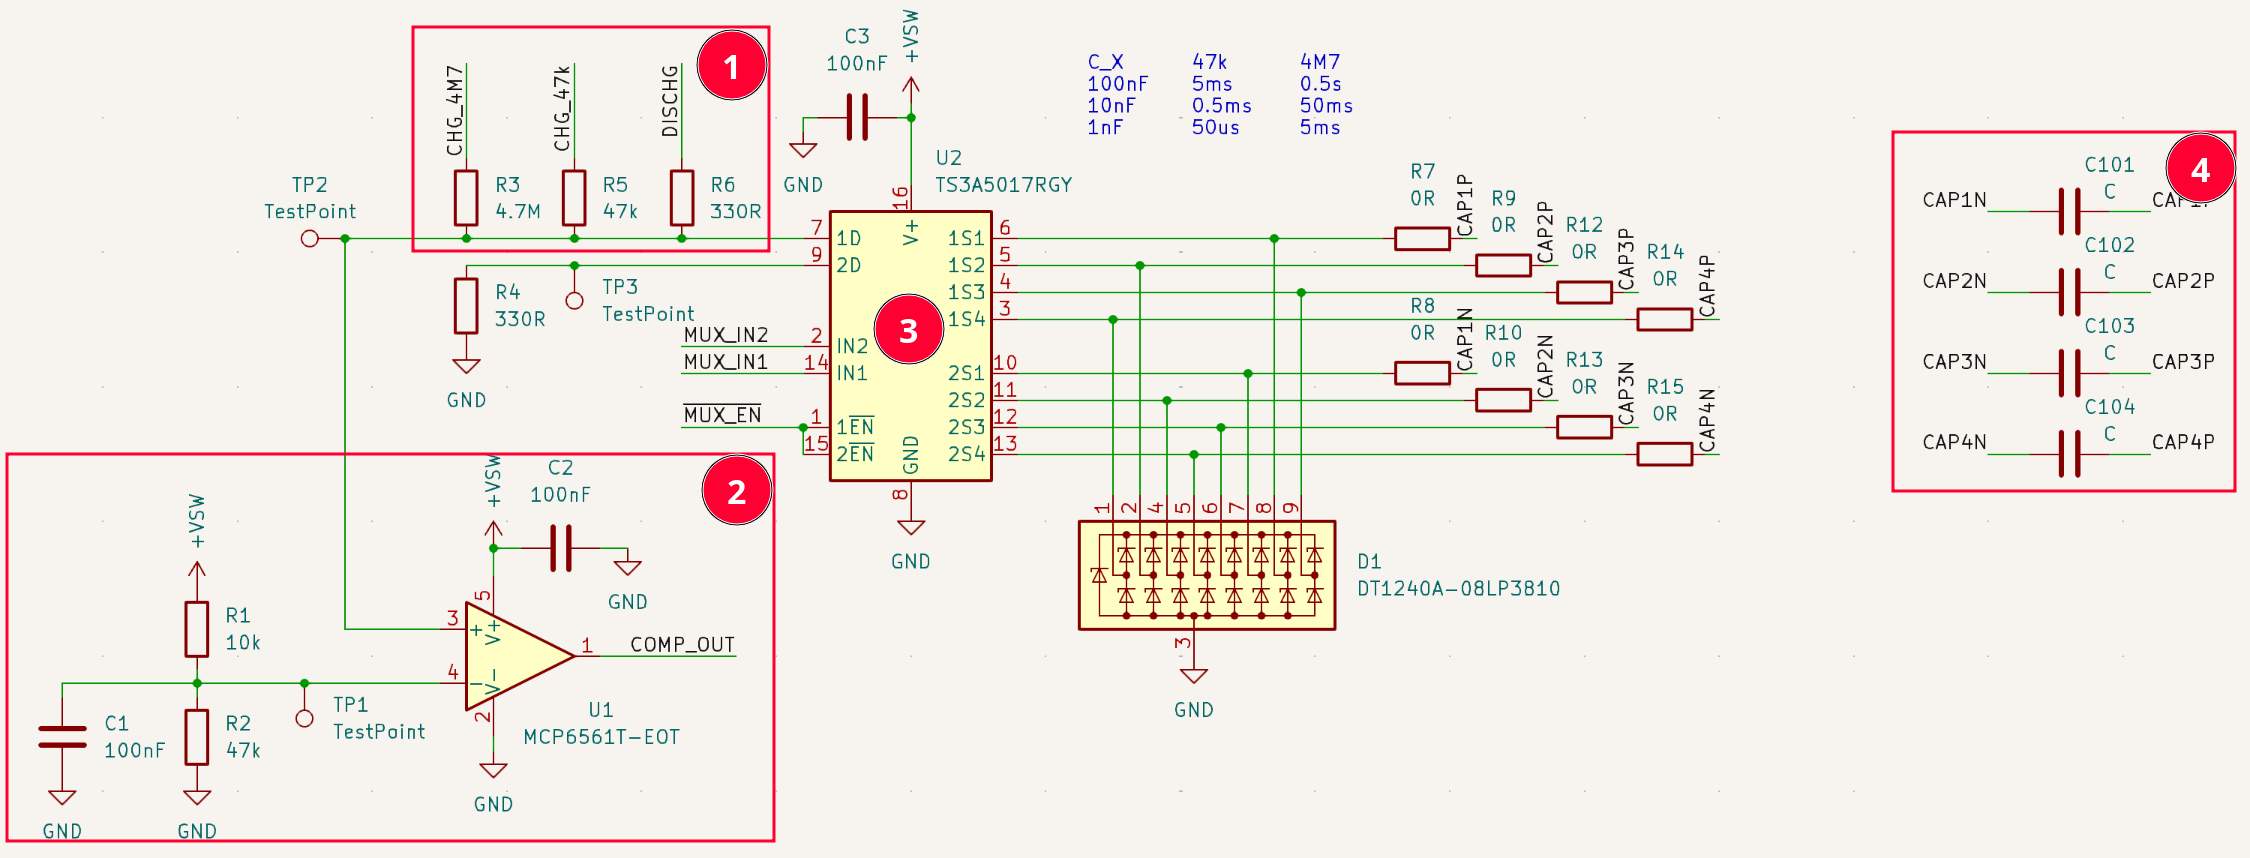
\includegraphics[width=.9\textwidth]{fig/sensor-measure-circuit.png}
    \caption{\label{fig:sensor-measure-circuit}The capacitance measuring circuit functions by charging the unknown capacitor $C_X$ through a known resistor $R_{CHG}$ and measuring the time it takes to reach a certain voltage derived from a voltage reference. The muxing (U2) and protection circuitry (D1) is also included. Resistors R7--15 are there to facilitate a complete isolation of the sensor from the measuring circuit, for measuring the capacitor elements externally, if the need be, without damaging the board. The full schematic is available in Appendix \ref{chapter:sensor-files}.}
\end{figure}

The capacitance can be calculated from readings obtained in Figure \ref{fig:cap-measure}. Given the charging voltage $U = 3.3~\mathrm{V}$ (it may not seem so from the Figure, due to the charging resistor being disconnected as soon as the threshold voltage is reached). The capacitance RC time constant is defined as
\begin{equation} %(7.6*10^-6)/(47*10^3)
    \tau = RC ~~~\rightarrow~~~ C = \dfrac{\tau}{R} = \dfrac{7.6 \cdot 10^{-6}}{47 \cdot 10^3} = 161~\mathrm{pF}.
\end{equation}
This result goes in line with the estimate given in Section \ref{section:expected-cap}. The reading would triple when submerged fully in water.

\begin{figure}[H]
    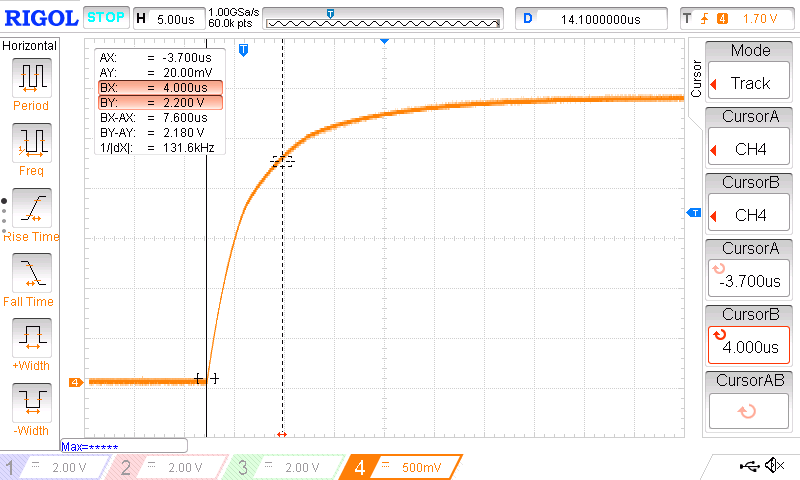
\includegraphics[width=.8\textwidth]{fig/cap-measure-inv.png}
    \caption{\label{fig:cap-measure}Sensor capacitor (in air) voltage rise time measurement when charged through a 47k$\Omega$ resistor, which was later replaced by a different value to increase the measuring time.}
\end{figure}

The original 47 k$\Omega$ and 4.7 M$\Omega$ resistors were replaced by 100 k$\Omega$ and 1 M$\Omega$ resistors to improve the measuring performance. These resistors were designed with this possibility in mind and a larger footprint was used to make this process easier. the 4.7 M$\Omega$ resistor was not able to charge the circuit up to the detecting threshold of the comparator, because the rest of the components incurred parasitic resistance to ground of about 15 M$\Omega$, forming a voltage divider.

This setup provides repeatable and stable measurements in free air and when the capacitor is completely submerged in water. It is sensitive enough to reliably detect close proximity (1 cm) or touch of a human hand.

The following code is responsible for each sample conversion, refer to the comments for principle explanation.
\newpage
\begin{lstlisting}
pub async fn sample_current_channel(
        &mut self, range: SoilSensorRange
    ) -> SoilSensorResult {
    /* 1. Handle the range selection by setting the required charge 
    pin as output and the unused pin as high-impedance input. */
    match range {
        SoilSensorRange::Low => {
            self.chg_1m.set_as_input(Pull::None);
            self.chg_100k.set_as_output(Speed::Low);
            self.chg_100k.set_low();
        },
        SoilSensorRange::High => {
            self.chg_100k.set_as_input(Pull::None);
            self.chg_1m.set_as_output(Speed::Low);
            self.chg_1m.set_low();
        },
    }
    /* 2. Bridge the connection between the selected capacitor 
    and the rest of the measuring circuit (the channel selection 
    happens before this function) and discharge the capacitor. */
    self.dischg.set_low();
    self.mux_nen.set_low();
    Timer::after_micros(100).await;
    /* Note: the DISCH pin is configured as open-drain output. */
    self.dischg.set_high();
    /* 3. Start charging the capacitor through the selected resistor. */
    match range {
        SoilSensorRange::Low => {
            self.chg_100k.set_high();
        },
        SoilSensorRange::High => {
            self.chg_1m.set_high();
        },
    }
    let start = Instant::now();
    /* 4. Await either the interrupt from the COMParator input
    or a timeout in case a wrong range was selected. */
    let ret = match select(
        self.comp.wait_for_high(), 
        Timer::after_millis(2)
    ).await {
        Either::First(_) => {
            /* 5a. Calculate the measured time to be returned 
            in case of successful conversion */
            let mut elapsed = start.elapsed();
            match range {
                SoilSensorRange::Low => {
                    elapsed *= 10;
                },
                SoilSensorRange::High => {
                    elapsed *= 1;
                },
            }
            SoilSensorResult::Ok(elapsed.as_micros() as u16)
        },
        /* 5b. Timeout */
        Either::Second(_) => SoilSensorResult::Timeout,
    };
    /* 6. Return all pins to default state */
    self.chg_100k.set_as_input(Pull::None);
    self.chg_1m.set_as_input(Pull::None);
    self.dischg.set_low();
    self.mux_nen.set_high();
    ret
}
\end{lstlisting}

\FloatBarrier
\section{\label{section:ota-implementation}Over--the--air Update Implementation}
It is the responsibility of the update process to securely and reliably transfer the binary image of the firmware from the host computer through the Gateway to the designated Node (sensor) of the network. 

This task is complicated by the limited resources available on embedded devices, as discussed in Section \ref{section:ota-update-support}, and the slow and sometimes unreliable nature of the wireless connection in general. Following sections describe the protocol solution to this aspect of the OTA update process.

The performance testing was done along with the range test described in the following Section \ref{section:range-test}.

\subsection{Data Fragmentation}
The binary needs to be fragmented in order to be transmitted piece by piece. To guarantee the assembly of these fragments on the Node, an acknowledge mechanism must be present along with a way to detect errors in the transferred data. While the LoRa physical layer provides forward error correction and also up to a 16 bit CRC checksum, the error rate is from experience still too high to be practical. To tackle this, a custom 32 bit CRC was used to protect each fragment together with a SHA256 hash of the whole assembled binary, which is calculated as the last step in the update process.

\begin{figure}[p]
    \includesvg[width=0.9\textwidth]{fig/ota-algo.drawio.svg}
    \caption{\label{fig:ota-algo}Simplified flowchart depicting the over--the--air update communication process between the Gateway and the Node.}
\end{figure}

Figure \ref{fig:ota-algo} provides a basic overview of the OTA update process. The communication with the host is left out for brevity, but mostly mirrors the operations that happen on the Gateway. Names in the cells correspond to packet types defined in the \link{https://github.com/manakjiri/lora-module-fw/blob/main/module-runtime/src/ota/common.rs}{module-runtime/src/ota/common.rs} file as \code{enum OtaPacket}. Packets are serialized and deserialized using the \link{https://docs.rs/postcard/latest/postcard/}{postcard} Rust package.

\subsection{Acknowledge Mechanism}
The Automatic Repeat Request (ARQ) mechanism is inspired by Selective Repeat ARQ. The receiver is able to accept frames that are out of order and selectively requests missing or corrupted blocks. In contrast to standard ARQ, here the acknowledge (ACK) packet contains up to 32 indexes of blocks that were successfully received, instead of just one.

Likewise, the transmitter does not expect to receive ACK packets consistently and continues to transmit in order for up to 16 unACKed frames. The receiver is thus able to relax the rate of ACK packets to reduce the air time usage. Since the transmitter is not attempting to use the maximum available channel capacity, it transmits about one packet per second, it does not need the immediate response to measure latency.

\subsection{Bootloader}
Once the data was transferred to the target Node to be updated, the Node needs to perform the update by swapping the old firmware image with the new one, as described in Section \ref{section:ota-update-support}. The Embassy Bootloader was used for this purpose, as it is easy to integrate, features small memory footprint of just 8 KBytes, along with a rollback feature \cite{embassy_project_documentation_bootloader_2024}. The rollback is initiated after device reset if the application failed to signal to the bootloader, that it started up successfully by writing a special value in the state section of the FLASH.

%!TEX ROOT=main.tex

\section{\label{section:range-test}LoRa Module Range and Link Speed Test}
In order to determine the real-world performance, a range test was conducted. Primary points of interest are
\begin{itemize}
    \item maximum practically usable range of the solution and connection quality deterioration as the distance and occlusion increases,
    \item performance of the designed module compared with the Nucleo development board as reference,
    \item the effect of proximity of the antenna to the ground and
    \item the effect of the spreading factor (SF) modulation parameter.
\end{itemize}

All testing so far was done in home environment with Nodes in close proximity and no major packet loss could be observed. Given the relatively low experience in RF design however, it is expected the module will perform worse than the Nucleo board.

With increasing spreading factor, the symbol time increases and the link budget goes with it, as can be seen in Table \ref{table:semtech-sf}. But longer symbol time relies on more stable and precise frequency reference. 

\begin{figure}[H]
    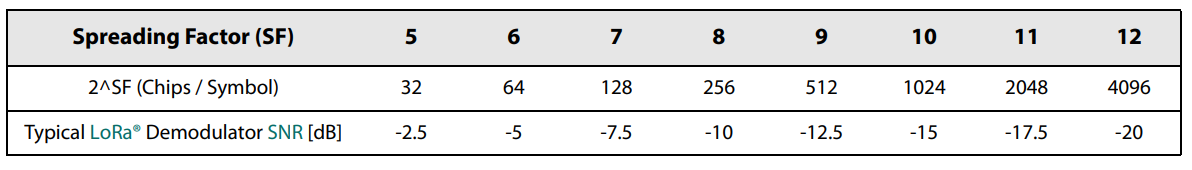
\includegraphics[width=\textwidth]{fig/semtech-sf-table.png}
    \caption{\label{table:semtech-sf}Range of Spreading Factors (SF).}
\end{figure}

Bandwidth variation exhibits similar traits, but to stay within the legal limits of the EU868 band, it is necessary to stay within $125\text{--}500~\mathrm{kHz}$ \cite{thethingsnetwork_eu863-870_nodate}. This is the reason for selecting SF as the variable, while keeping the Bandwidth and the coding rate (CR) constant. CR also has a very predictable effect on the connection quality.

\subsection{Hypothesis}
It is expected the proximity to the ground will have high impact on the usable range of the sensor, meaning Nodes mounted with their antenna closer to the ground should perform worse. Higher SF should yield longer range. We are not expecting to surpass distance of $1~\mathrm{km}$.

\subsection{\label{section:range-prerequisite}Prerequisite}
The maximum achievable SF needed to be determined. This was done experimentally, starting with SF5 and incrementing util it was no longer possible to transfer data. This test was conducted using Nucleo acting as the initiator of connection with the LoRa module. Devices were situated on a desk about 1.5 meters apart with their antennae positioned orthogonally in respect to each other to avoid overwhelming the receiver. All other parameters are identical to those used in the latter experiment.

The connection was stable at SF11, but at SF12 the LoRa module stopped responding, thus the experiment was done at SF5 and SF11, which corresponds to a theoretical delta of $15~\mathrm{dB}$.

\subsection{Methodology}
All LoRa modulation and packet parameters were set in firmware (commit \link{https://github.com/manakjiri/lora-module-fw/tree/76acdcd7b31f259c88f1808ed79886dc26295b4e}{76acdcd}) identically for all devices used, a summary is provided in Table \ref{table:range-test-parameters}. 

\begin{table}[H]
\begin{center}
\caption{\label{table:range-test-parameters}LoRa parameters for range testing.}
    \begin{tabular}{|l|l|} \hline
    Frequency             & $869.525~\mathrm{MHz}$\\ \hline
    RF power output       & $15~\mathrm{dBm}$\\ \hline
    Bandwidth             & $250~\mathrm{kHz}$\\ \hline
    Coding rate           & $4:8$ (2x overhead) \\ \hline
    Bandwidth             & $250~\mathrm{kHz}$\\ \hline
    Preamble length       & $32~\mathrm{b}$\\ \hline
    Implicit header       & No\\ \hline
    LoRa CRC              & No\\ \hline
    Inverted IQ           & No\\ \hline
    Transmit boost        & No\\ \hline
    Receive boost         & No\\ \hline
    \end{tabular}
\end{center}
\end{table}

LoRa modules used the MOLEX 105262--0003 antenna and Nucleo boards used their stock antenna, all were close to vertical orientation. A pole with two LoRa modules and one Nucleo (see Figure \ref{fig:range-nodes}) was constructed to act as the stationary set of Nodes to test against. Another Nucleo board was attached to a car (see Figure \ref{fig:range-gateway}) to act as the Gateway, see Table \ref{table:range-test-devices} for more details.

\begin{figure}[p]
    \centering
    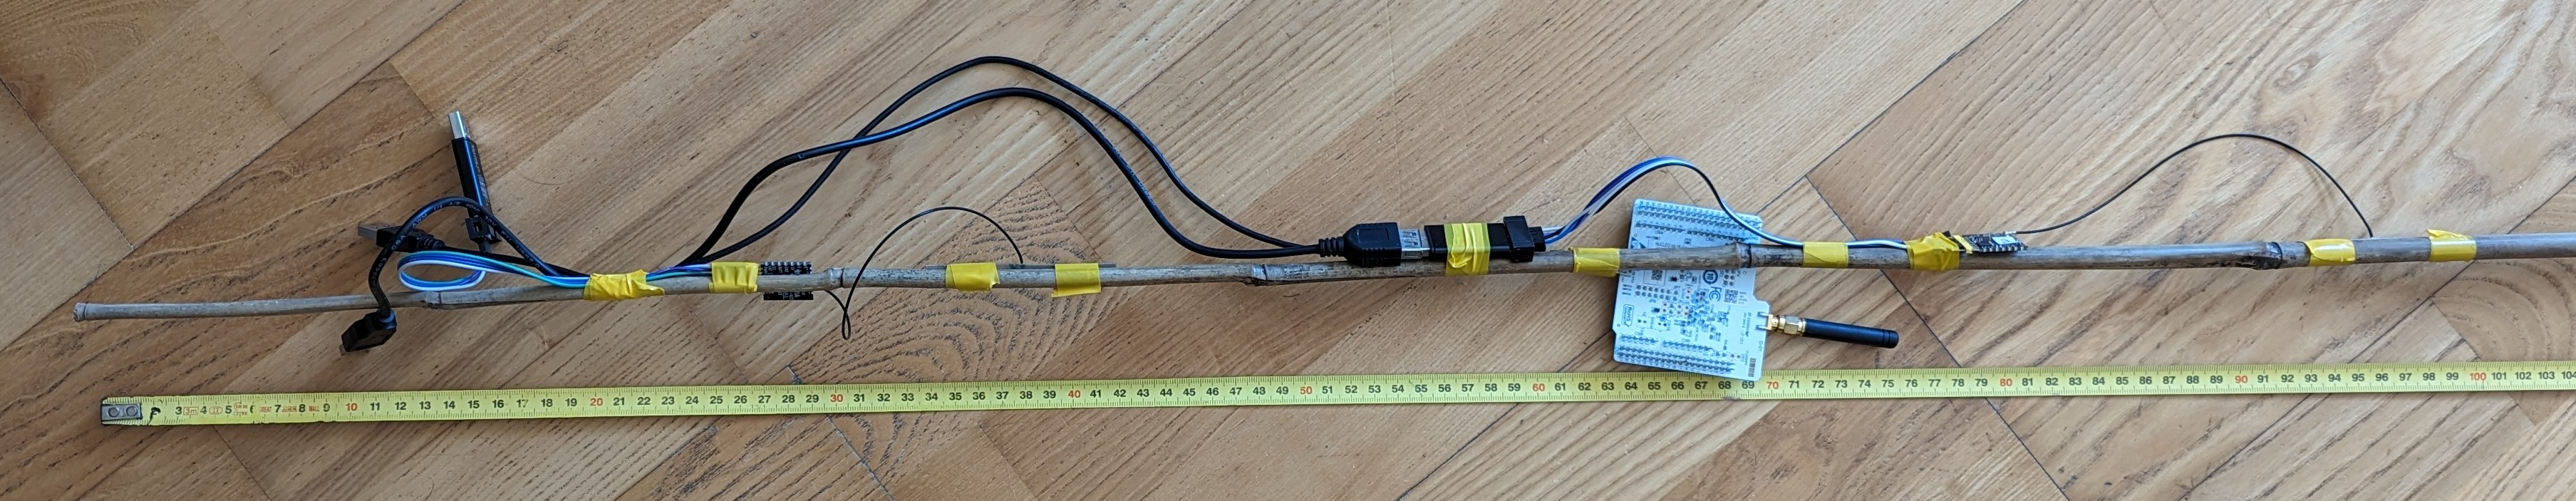
\includegraphics[width=.9\textwidth]{img/lora-pole.jpg}\vspace{1em}
    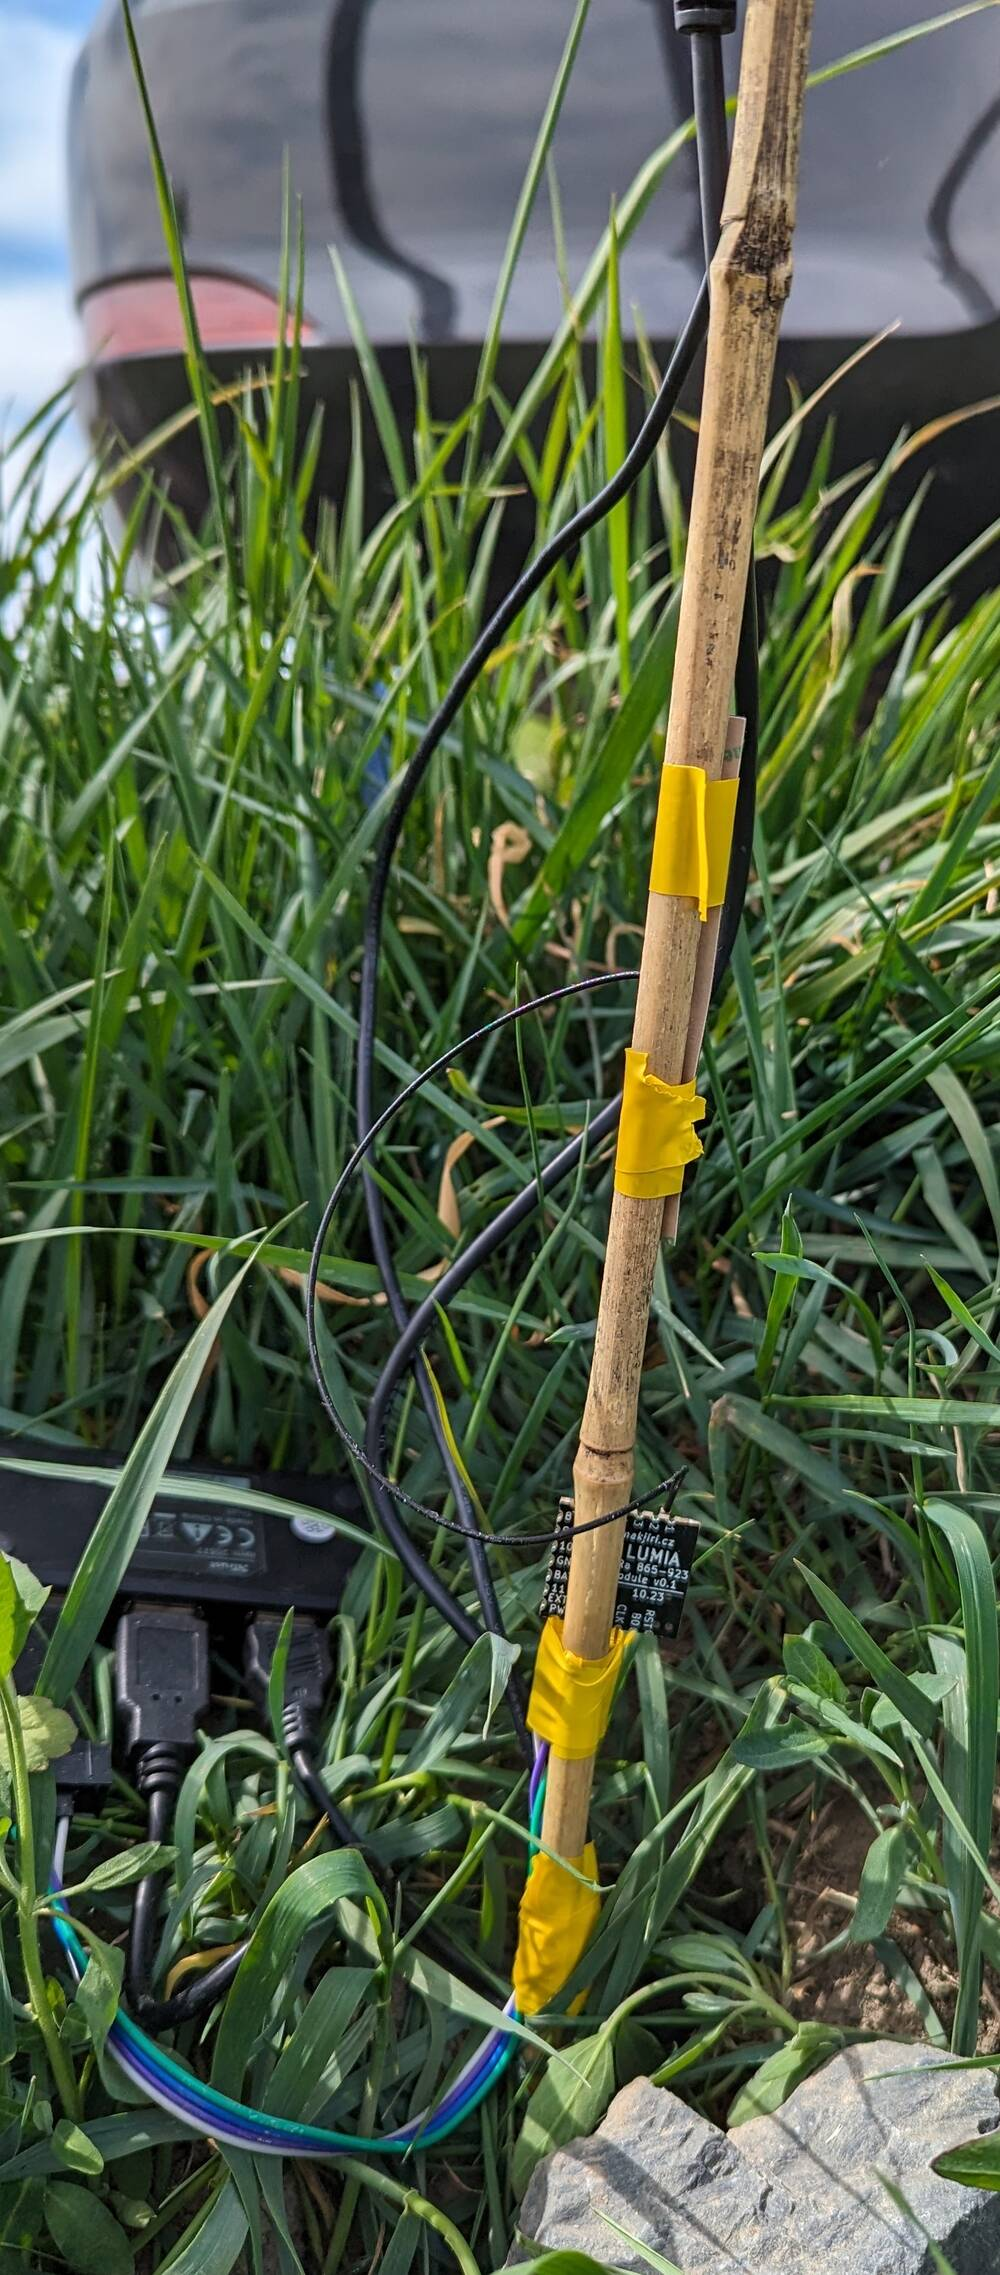
\includegraphics[width=.25\textwidth]{img/range-pole-base.jpg}\hfil
    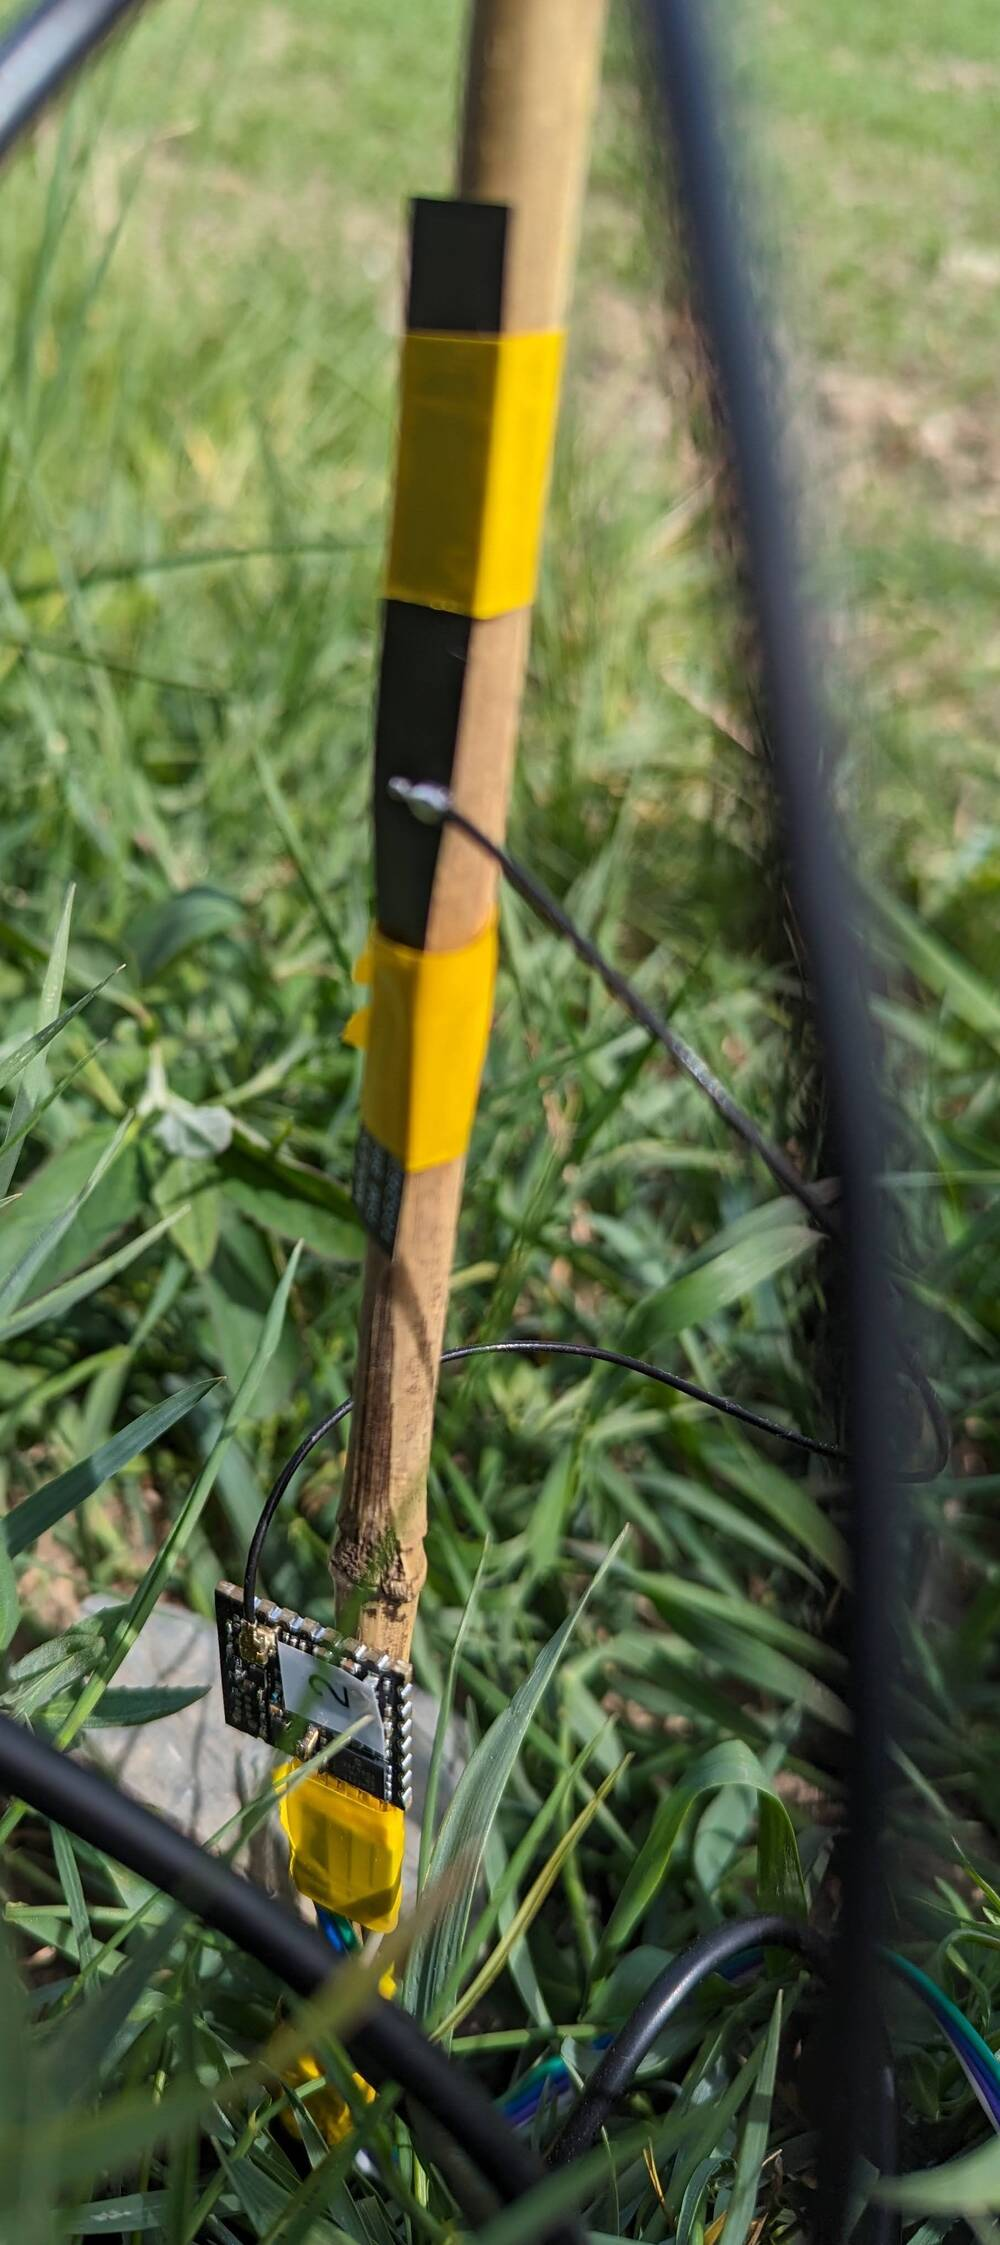
\includegraphics[width=.25\textwidth]{img/range-pole-bottom.jpg}\hfil
    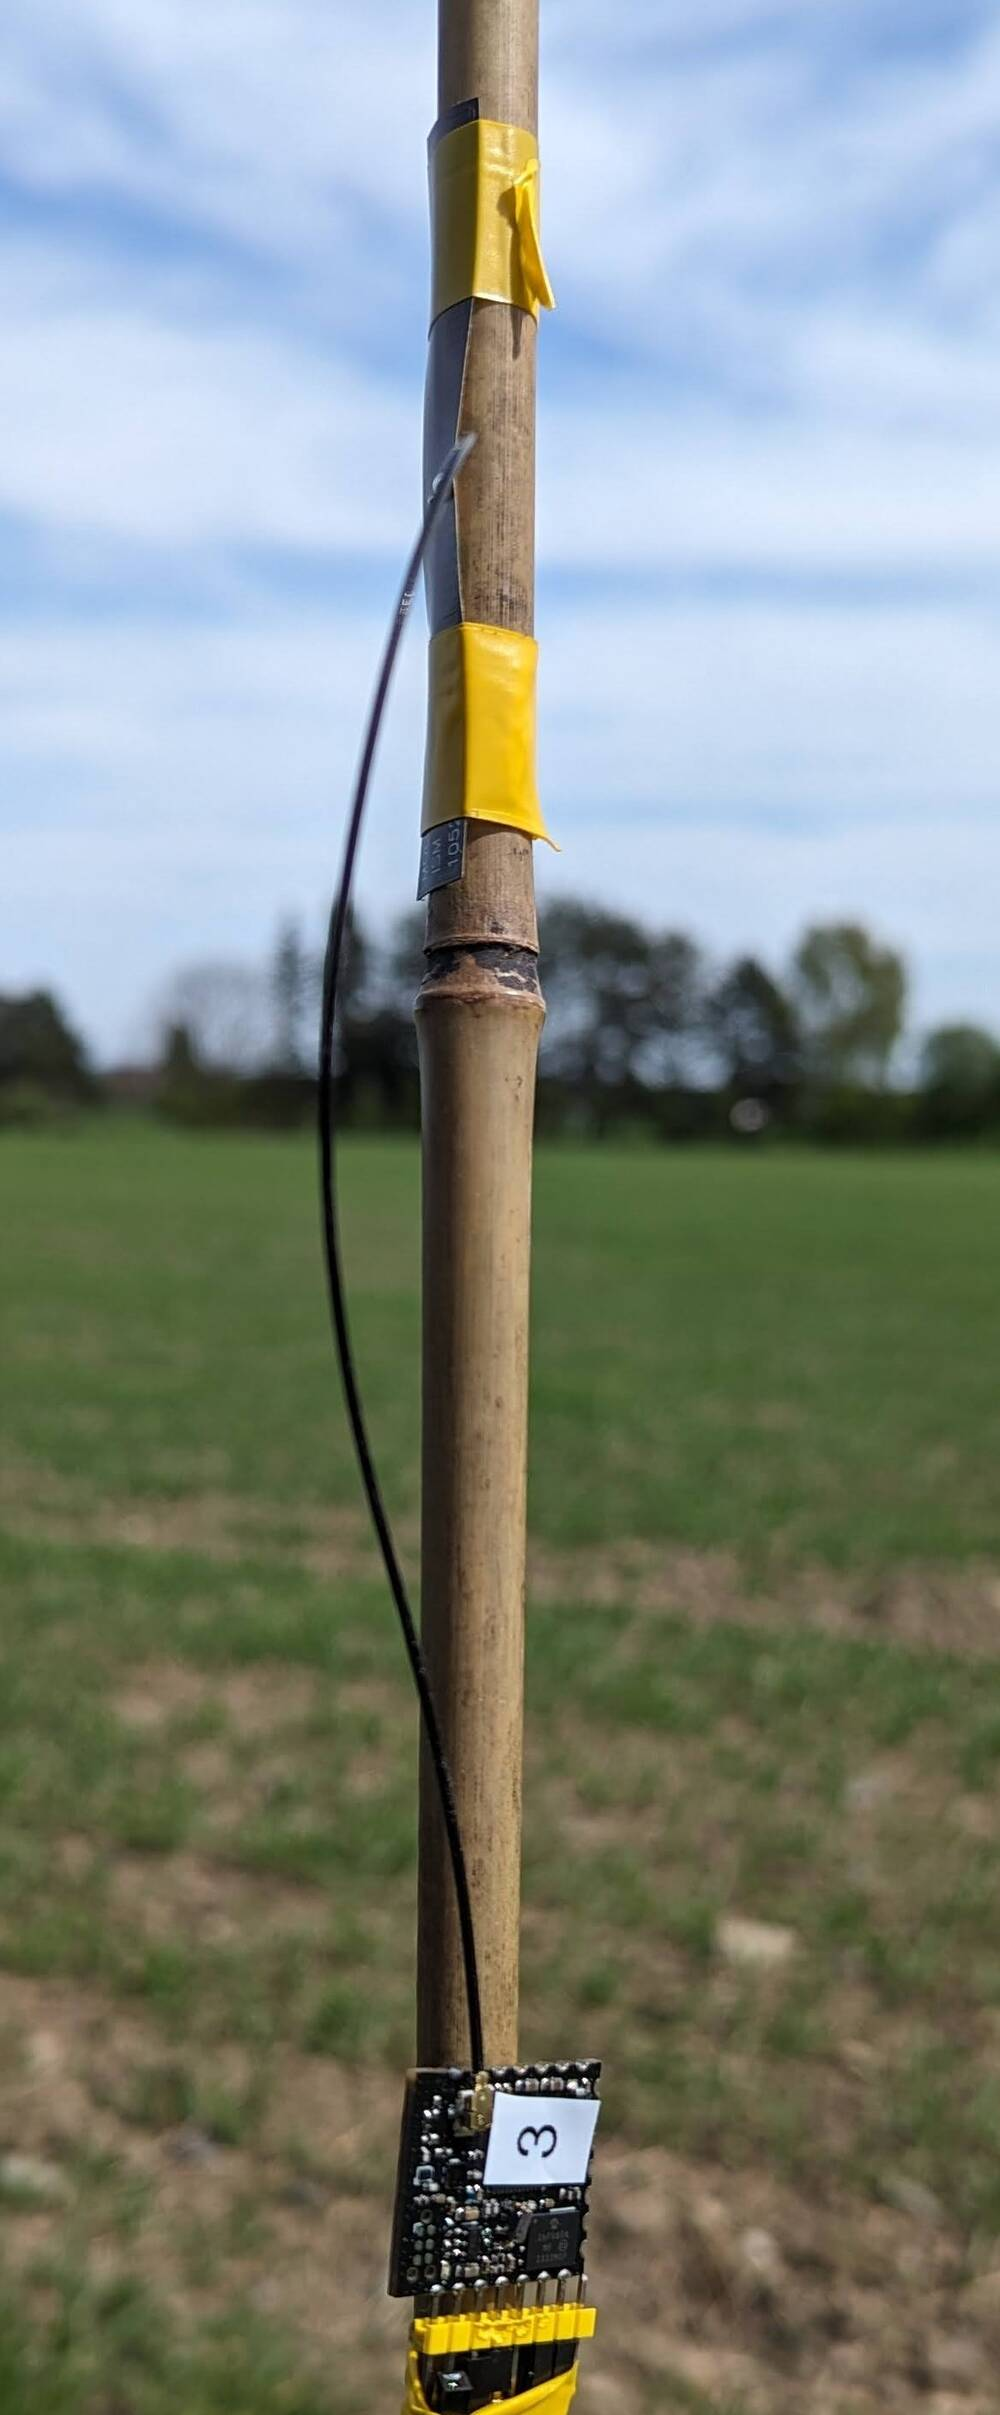
\includegraphics[width=.24\textwidth]{img/range-pole-top.jpg}
    \caption{\label{fig:range-nodes}Close-up of the pole with Nodes attached for range testing.}
\end{figure}

\begin{figure}[p]
    \centering
    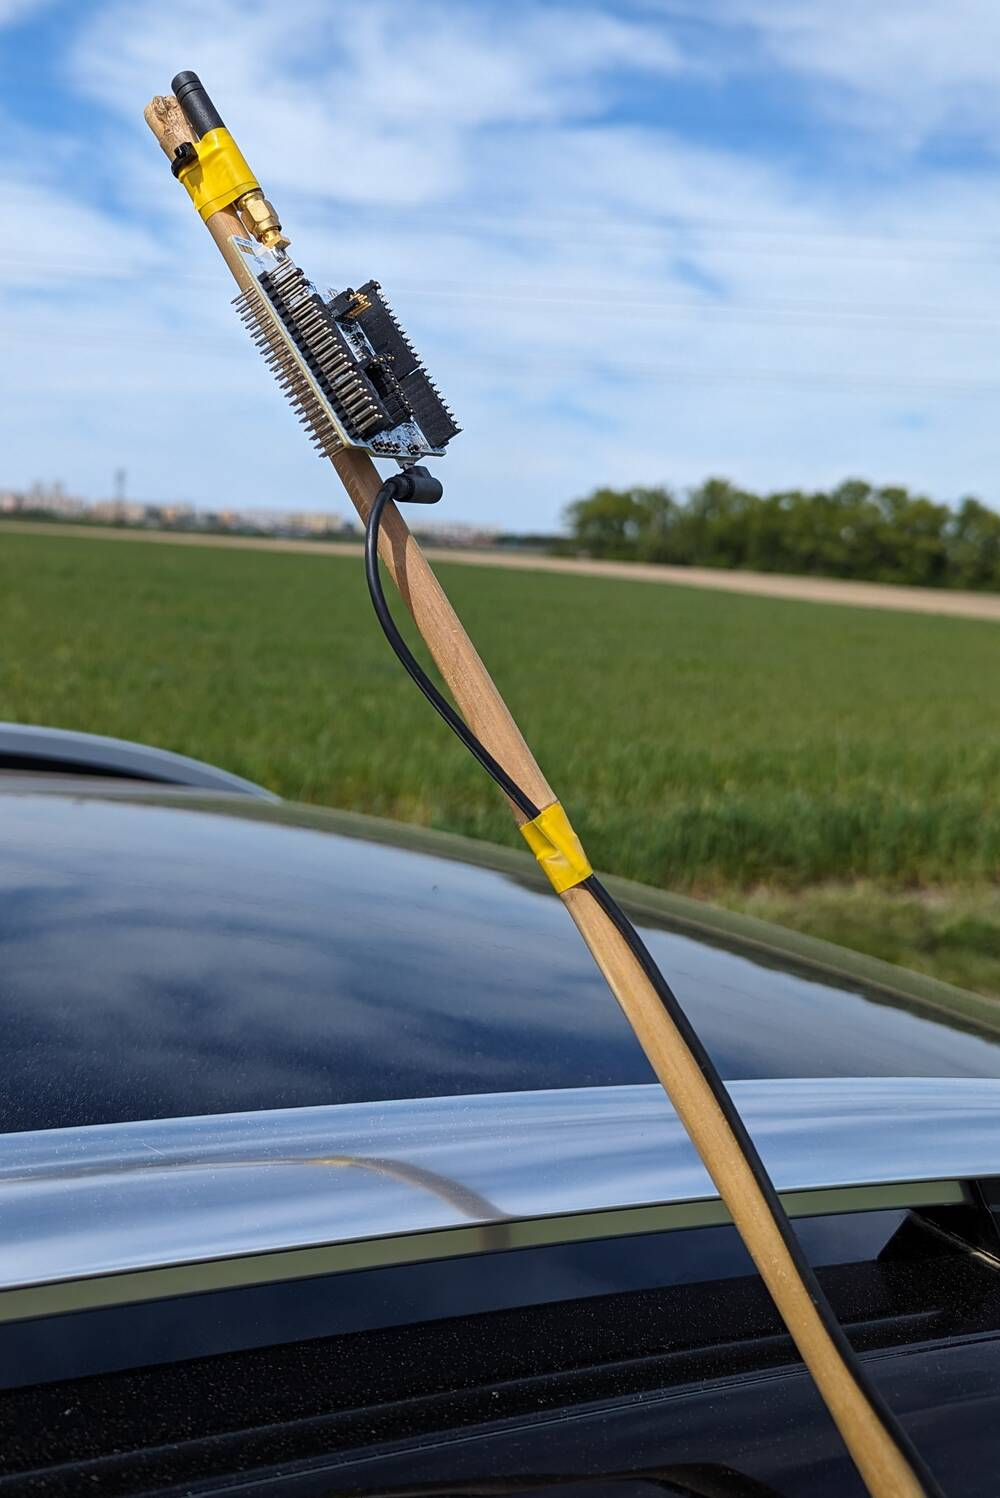
\includegraphics[width=.35\textwidth]{img/range-gateway1.jpg}\hfil
    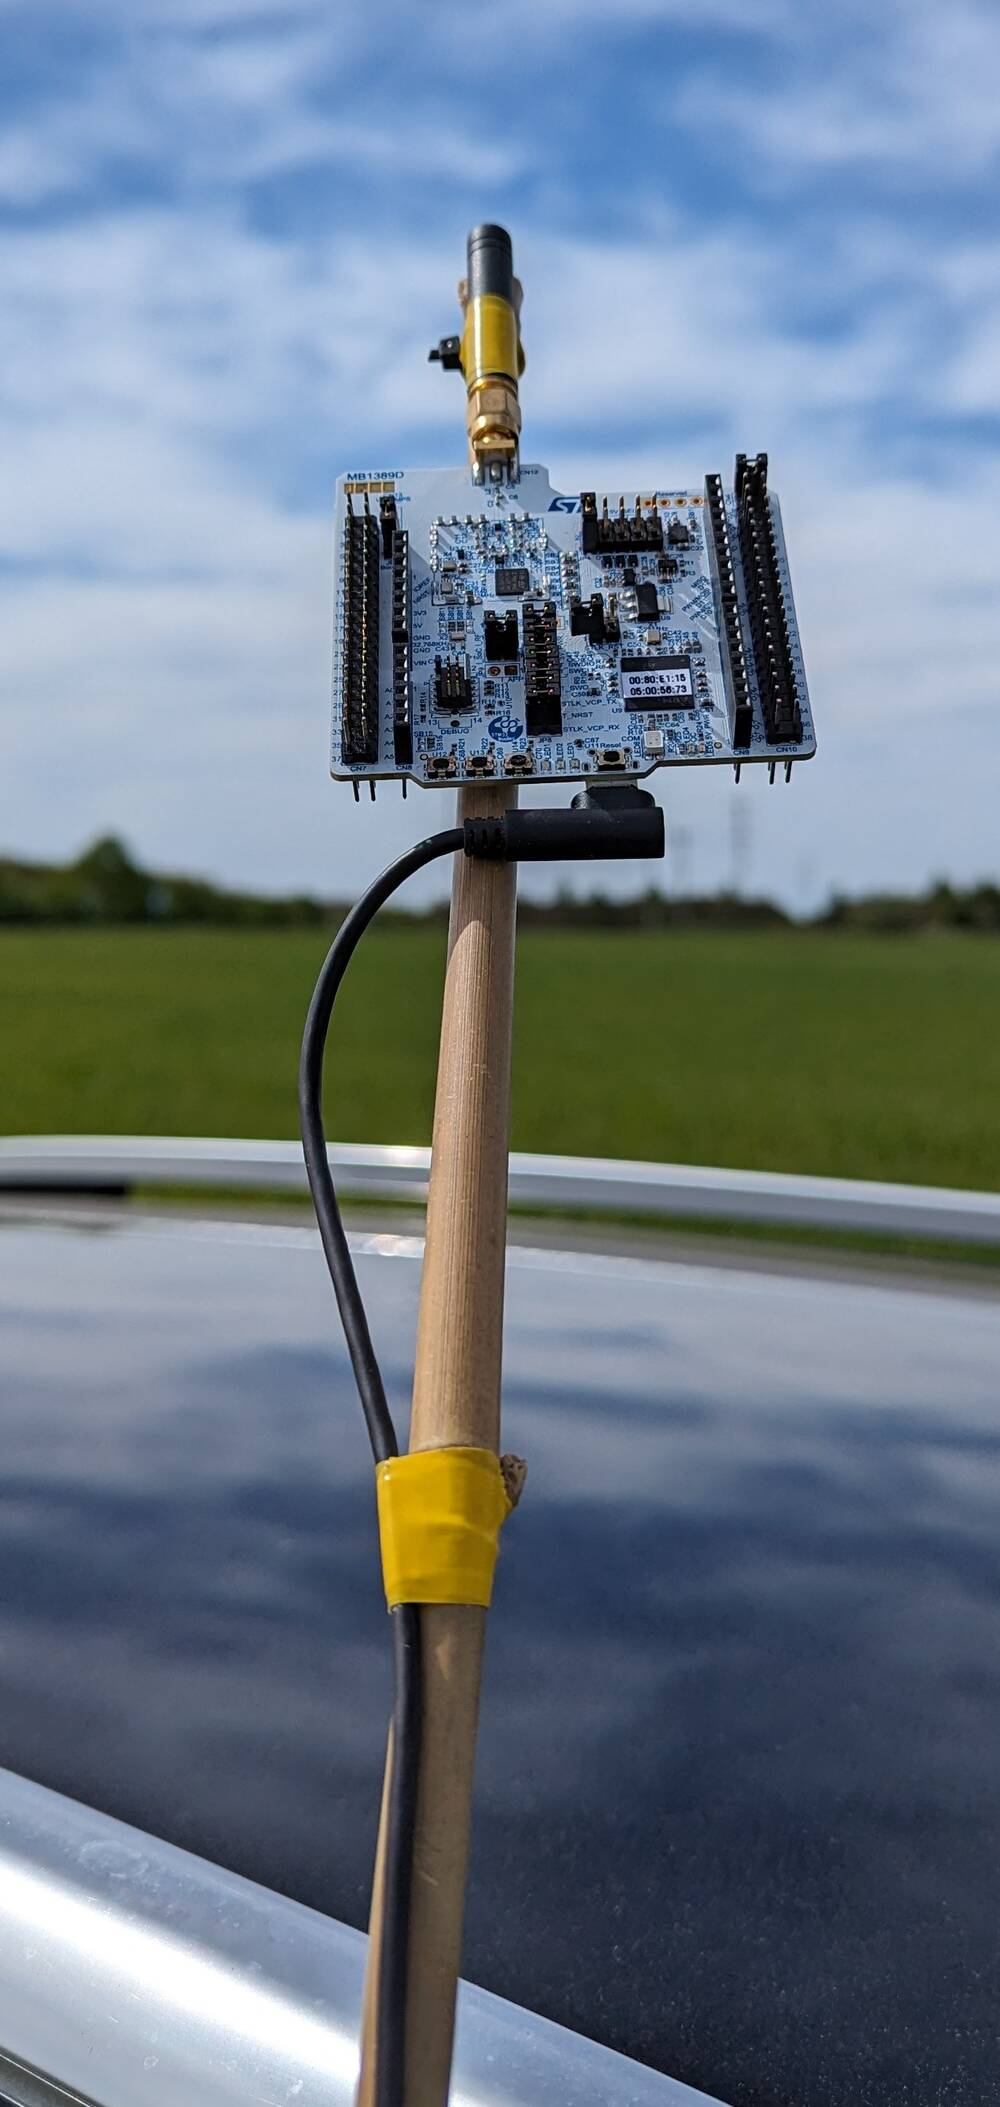
\includegraphics[width=.25\textwidth]{img/range-gateway2.jpg}
    \caption{\label{fig:range-gateway}Close-up of Nucleo attached to the car acting as the Gateway for range testing.}
\end{figure}

\begin{table}[H]
\begin{center}
\caption{\label{table:range-test-devices}Devices used for range testing.}
    \begin{tabular}{|l|l|l|} \hline
    \textbf{Device} & \textbf{Height\footnote{Measured distance from the root of the antenna to ground level} [m]} & \textbf{Address}\footnote{Data presented will use these addresses to distinguish between the different Nodes used in the experiment} \\ \hline
    Nucleo (Gateway) & 1.65 & 1 \\ \hline
    LoRa module (Node) & 0.19 & 2 \\ \hline
    Nucleo (Node) & 0.55 & 4 \\ \hline
    LoRa module (Node) & 0.82 & 3 \\ \hline
    \end{tabular}
\end{center}
\end{table}

A location was picked to represent the final use--case, a field with sections of direct line--of--sight (LOS) and sections obstructed by hills. This place is situated near Průhonice municipality in the Czech Republic. The pole with Nodes attached was installed at \href{https://en.mapy.cz/letecka?q=50.0012006N%2C%2014.5308962E&x=14.5381677&y=50.0011824&z=16}{50.0012006N, 14.5308961E}\footnote{https://en.mapy.cz/letecka?q=50.0012006N\%2C\%2014.5308962E\&x=14.5381677\&y=50.0011824\&z=16} (WGS84).

A set of measurements was taken through the Gateway at different locations progressing further from the stationary pole with the Nodes attached. These measurements consisted of downloading a random binary 1 KB file to each of the Nodes consecutively. This file was fragmented on the fly by the OTA update protocol to 16 blocks of 64 bytes each.

This means that effectively 16 different measurements of the signal quality were taken at each location for each of the three Nodes. Measurements were recorded by the system in a CSV file containing the time since download started, the amount of packets sent and the last block that was acknowledged - thus a success rate can be calculated. In case the download failed to initiate, nothing gets recorded and that is interpreted as 0\% success rate.

\subsection{Results}
As this is an experiment, where direct line--of--sight cannot be relied upon to interpret the results, it was deemed necessary to somehow capture the environment, the terrain, and present it along with the obtained data.

Altitude data was obtained from the \link{https://api.mapy.cz/v1/elevation}{Seznam.cz elevation API} in 5 m resolution of interpolated coordinates of lines connecting the Nodes and Gateway locations. This location data is also available in raw form as part of the Appendix \ref{chapter:more-range-test}.

\subsubsection{\label{section:edsl-definition}Elevation Deviation from the Straight Line}
Following graphs describe the terrain in terms of Elevation Deviation from the Straight Line (EDSL) connecting the Nodes location (spot 0) with the furthest point at which the last measurement was taken. Units of EDSL proportionally translate to meters, since the effect is similar to subtracting the offset signal in data.

The same data without the EDSL interpretation is included as Appendix \ref{chapter:more-range-test} for completeness. It also demonstrates the need for such data manipulation, because the features of the terrain are a lot less apparent in the original data.

\begin{figure}[p]
    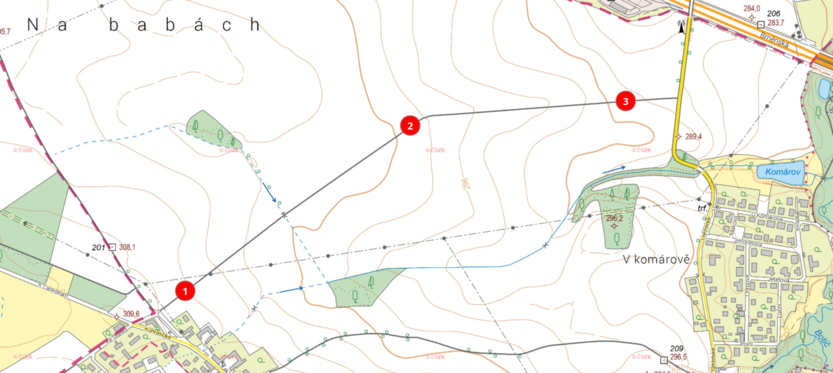
\includegraphics[width=.9\textwidth]{img/range-test-map.png}
    \caption{\label{fig:range-test-map}Map of the range test site. Correlation with Figures \ref{fig:range-relief} and Table \ref{table:range-results} follows: point 1 corresponds to the Nodes location (spot 0), point 2 is the spot 5 in both SF5 and SF11 measurements, point 3 is the spot 9 and spot 11 for SF11 and SF5 respectively. Source: \href{https://ags.cuzk.cz/geoprohlizec}{Geoprohlížeč ČÚZK}.}
\end{figure}

\subsubsection{Effect of the Spreading Factor}
Lower SF decreases the packet air time at the expanse of lower range reached. SF5 averaged $0.125~\mathrm{s}$, while SF11 averaged $1.125~\mathrm{s}$ round-trip time (excluding packet-loss) with these payloads.

Using SF5, it was possible to maintain stable connection with Nodes (3 and 4) positioned higher above the ground level even when occluded by the terrain. Connection with Node 2 was lost as soon as any occlusion was introduced. It can be expected that this setup would be feasible in very flat environments, but could be susceptible to dropouts with slight changes, such as growing crops.

The SF11 configuration exceeded expectations in terms of distance reached, a stable connection was maintained with all Nodes without difference in packet loss, which is perhaps most surprising, since some degradation was expected at least for the Node 2 position closest to the ground level. 

While the range was higher than with SF5, the connection quality is somewhat worse in the stable regions (less than 500 m distance, direct line-of-sight) for SF11. This suggests that a stability limit was indeed reached, as alloted to in the Prerequisite Section \ref{section:range-prerequisite}.

\begin{figure}[p]
    \centering
    \subfloat[SF11]{\includesvg[width=0.95\textwidth]{data/range/out/relief-sf11.svg}} \hfil
    \subfloat[SF5]{\includesvg[width=0.95\textwidth]{data/range/out/relief-sf5.svg}}
    \caption{\label{fig:range-relief}Graph of the range test locations, their distance from the pole with Nodes, and the relief in the path of the signal described as Elevation Deviation from the Straight Line \ref{section:edsl-definition}, which compensates the downward slope of the terrain and brings attention to the features of the terrain. Black crosses signify the position of the antennae of each device for each spot number.}
\end{figure}

\begin{figure}[p]
    \centering
    \subfloat[SF11]{\includesvg[width=\textwidth]{data/range/out/success-sf11.svg}} \hfil
    \subfloat[SF5]{\includesvg[width=\textwidth]{data/range/out/success-sf5.svg}}
    \caption{\label{fig:range-results}Graph of the packet transfer success rate for each Node with respect to the transmission distance.}
\end{figure}

\begin{figure}[p]
\begin{minipage}[t]{.45\textwidth}
    \vspace{0pt}
    \begin{tabular}{|l|l|l|l|}
\multicolumn{4}{c}{\textbf{SF11}} \\ \hline 
\textbf{Spot} & \textbf{Node 4} & \textbf{Node 3} & \textbf{Node 2} \\ \hline
0 & 100\% & 100\% & 100\% \\ \hline
1 & 100\% & 100\% & 100\% \\ \hline
2 & 100\% & 94\% & 100\% \\ \hline
3 & 100\% & 100\% & 100\% \\ \hline
4 & 100\% & 100\% & 100\% \\ \hline
5 & 100\% & 94\% & 100\% \\ \hline
6 & 100\% & 100\% & 94\% \\ \hline
7 & 100\% & 100\% & 100\% \\ \hline
8 & 94\% & 100\% & 100\% \\ \hline
9 & 100\% & 94\% & 100\% \\ \hline
\end{tabular}

\end{minipage}
\begin{minipage}[t]{.45\textwidth}
    \vspace{0pt}
    %\begin{table}
        \begin{tabular}{|l|l|l|l|}
\multicolumn{4}{c}{\textbf{SF5}} \\ \hline 
\textbf{Spot} & \textbf{Node 4} & \textbf{Node 3} & \textbf{Node 2} \\ \hline
0 & 100\% & 100\% & 100\% \\ \hline
1 & 100\% & 100\% & 100\% \\ \hline
2 & 100\% & 100\% & 100\% \\ \hline
3 & 100\% & 100\% & 100\% \\ \hline
4 & 100\% & 100\% & 100\% \\ \hline
5 & 100\% & 100\% & 100\% \\ \hline
6 & 100\% & 100\% & 100\% \\ \hline
7 & 100\% & 100\% & 0\% \\ \hline
8 & 100\% & 100\% & 0\% \\ \hline
9 & 100\% & 100\% & 0\% \\ \hline
10 & 89\% & 0\% & 0\% \\ \hline
11 & 89\% & 100\% & 0\% \\ \hline
\end{tabular}
    
    %\end{table}
\end{minipage}
\caption{\label{table:range-results}Success rates for each node and location at spreading factors 5 and 11.}
\end{figure}

\begin{figure}[p]
    \centering
    \begin{minipage}[t]{\textwidth}
        \centering
        \begin{tabular}{|l|l|l|l|}
\multicolumn{4}{c}{\textbf{SF11-FAR1}} \\ \hline 
\textbf{Spot} & \textbf{Node 4} & \textbf{Node 3} & \textbf{Node 2} \\ \hline
0 & 100\% & 100\% & 100\% \\ \hline
10 & 100\% & 6\% & 0\% \\ \hline
\end{tabular}

        \vspace{1em}
    \end{minipage}
    \includesvg[width=\textwidth]{data/range/out/relief-sf11-far1-lines.svg}
    \caption{\label{fig:range-relief-far1}Table of the success rates and graph of the first long range test location, distance from the pole with Nodes, and the relief in the path of the signal described as Elevation Deviation from the Straight Line \ref{section:edsl-definition}, which compensates the downward slope of the terrain and brings attention to the features of the terrain. Black crosses signify the position of the antennae of each device for each spot number. Dashed lines highlight the direct line-of-sight for the antennae.}
\end{figure}

\begin{figure}[p]
    \centering
    \begin{minipage}[t]{\textwidth}
        \centering
        \begin{tabular}{|l|l|l|l|}
\multicolumn{4}{c}{\textbf{SF11-FAR2}} \\ \hline 
\textbf{Spot} & \textbf{Node 4} & \textbf{Node 3} & \textbf{Node 2} \\ \hline
0 & 100\% & 100\% & 100\% \\ \hline
11 & 100\% & 100\% & 100\% \\ \hline
\end{tabular}

        \vspace{1em}
    \end{minipage}
    \includesvg[width=\textwidth]{data/range/out/relief-sf11-far2-lines.svg}
    \caption{\label{fig:range-relief-far2}Table of the success rates and graph of the second long range test location, distance from the pole with Nodes, and the relief in the path of the signal described as Elevation Deviation from the Straight Line \ref{section:edsl-definition}, which compensates the downward slope of the terrain and brings attention to the features of the terrain. Black crosses signify the position of the antennae of each device for each spot number. Dashed lines highlight the direct line-of-sight for the antennae.}
\end{figure}

\subsubsection{Maximum Distance}
Finding the limit at FS11 proved to be more difficult than anticipated. The surrounding environment either contained too favorable, or absolutely unfavorable conditions at further distances. Two additional data points displayed in Figures \ref{fig:range-relief-far1} and \ref{fig:range-relief-far2} were gathered at locations outside of the planed path.

The first Figure \ref{fig:range-relief-far1} shows the only flawless connection with the Nucleo Node 4, which must have been facilitated thanks to a signal reflection from some other feature in the environment. While the connection with Node 3 was initiated and it acknowledged 2 packets, the connection later timed out after the Node failed to respond in 30 more attempts.

The second location, captured by Figure \ref{fig:range-relief-far2}, exhibited flawless transmission of the payload for all 3 Nodes at a distance of 1.2 km with occlusion.

The nature of LoRa is that it performs well within its large link budget, but once that is exhausted, the performance drops off rapidly. The attenuation of the medium through which the electromagnetic wave travels changes with temperature and saturation with humidity and particulate, the position of the antennae may change slightly due to wind and the onboard oscillators can drift with temperature and power supply.

Most of these factors remained constant throughout this experiment, since it was done within a 1.5 hour window, but must be considered for long-term deployments.

\section{\label{section:sensor-validation}Soil Moisture Sensor Validation}
A practical experiment was conducted to validate the functioning of the soil moisture sensor itself.

\begin{figure}
    \centering
    \subfloat[Illustrative picture]{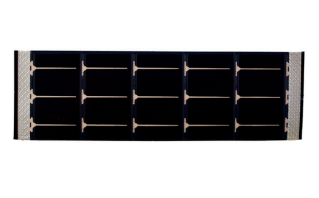
\includegraphics[width=.39\textwidth,angle=90]{img/panel.png}} \hfill
    \subfloat[IV Curve]{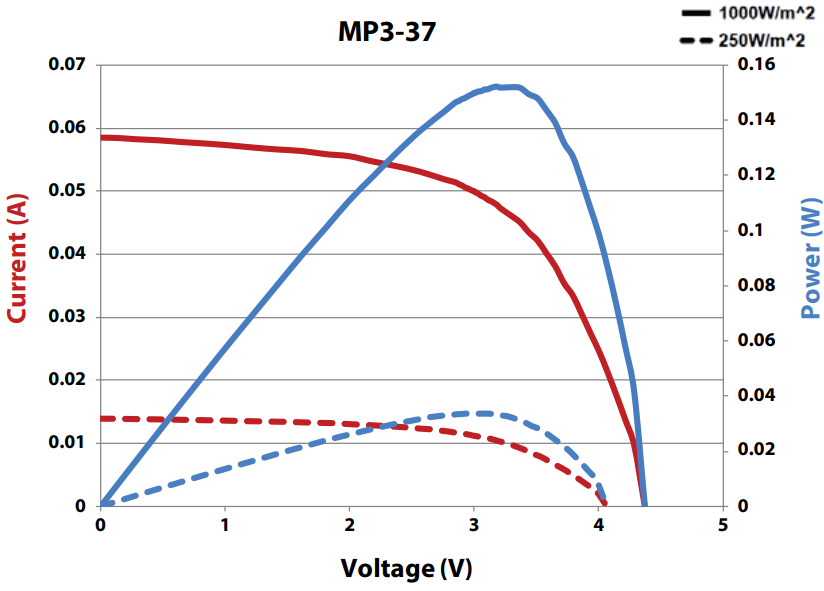
\includegraphics[width=.6\textwidth]{fig/panel-iv.png}}
    \caption{\label{fig:panel}The MP3-37 solar panel manufactured by PowerFilm, which was used for the soil moisture sensor validation.}
\end{figure}

\begin{figure}
    \centering
    \subfloat[Soil moisture sensor stuck in the pot (center) on a window sill faceing south. The lithium battery is connected externally through the raspberry pi pico development board (bottom), acting as a data logger of the voltage and current.]{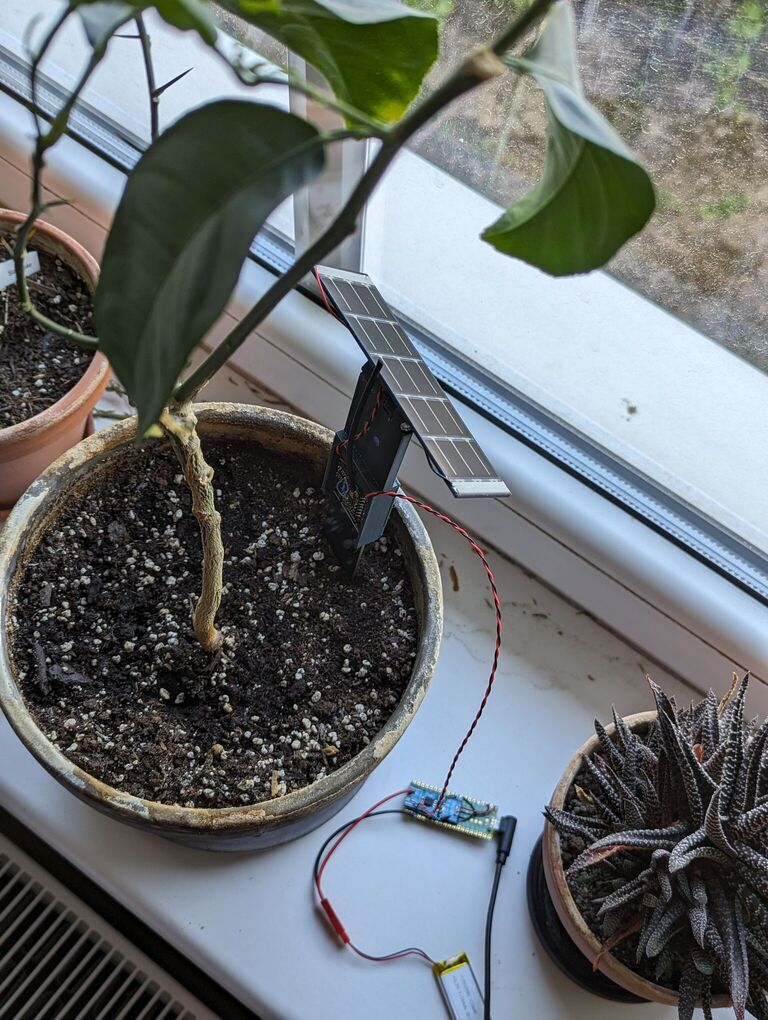
\includegraphics[width=.45\textwidth]{img/sensor-deploy-up.jpg}} \hfil
    \subfloat[Closeup picture of the sensor and its housing. The LoRa module is clearly visible, along with the conncetions to the solar panel, the battery and the antenna.]{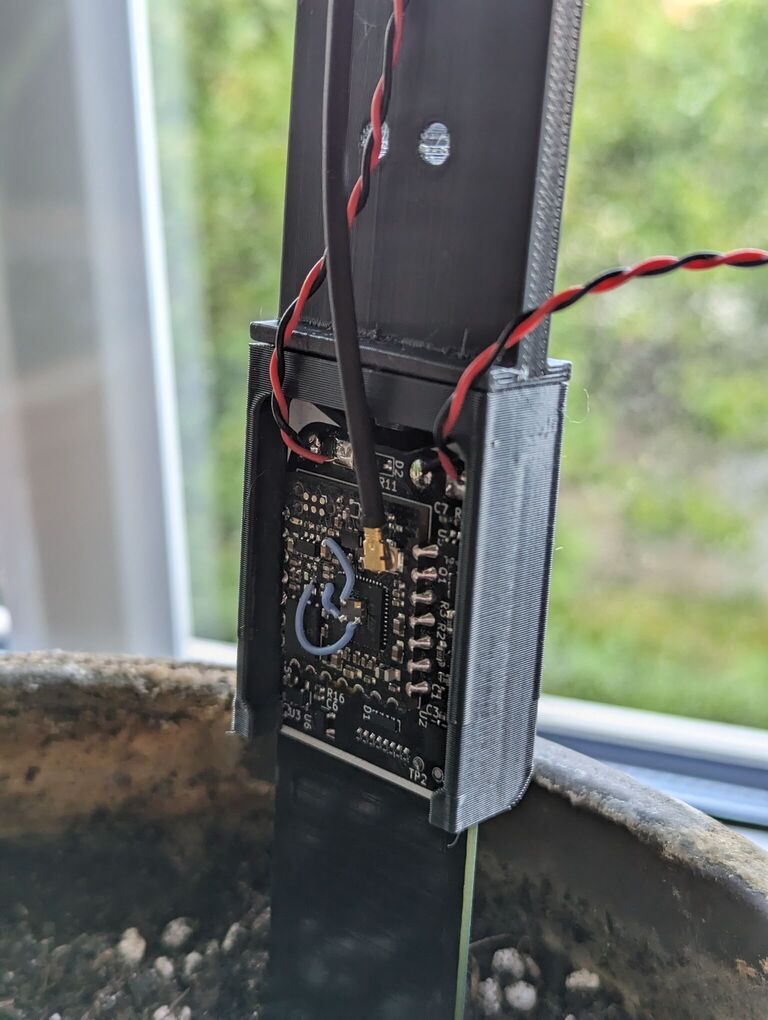
\includegraphics[width=.45\textwidth]{img/sensor-deploy-close.jpg}}
    \caption{\label{fig:sensor-deploy}Soil moisture sensor proof--of--concept deployment scenario used for validating the solar panel performance and the sensor's measuring capabilities.}
\end{figure}

\subsection{Hypothesis}
The sensor should detect soil moisture based on the experiments done during sensor validation. It is also expected that the sensor will be able to charge its battery when enough sunlight is available.

\subsection{Prerequisite}
The sensor is meant to be made self--sufficient thanks to a solar panel. The main constraint is the power generated and the panel's dimensions. Since the solar panel is charging the battery directly, it needs to generate sufficiently high voltage to do so. The MP3--37 from PowerFilm was picked, because its open circuit voltage is 4.6 V, and according to \ref{fig:panel}, it should produce 50 mA at 4.1 V, which is ideal for this application.

%https://cz.mouser.com/datasheet/2/1009/Electronic_Component_Spec_Sheet_Cla_77DEA84523C82-1658524.pdf

A sensor housing needs to be constructed to support the solar panel in the correct orientation. The housing was designed in Fusion 360 CAD software and 3D printed, visible in Figure \ref{fig:sensor-deploy}. The housing has a support arm for the solar panel, which allows it to swivel.

\subsection{Methodology}
The sensor was stuck in the existing planter of a citrus tree plant. Sensor readings are gathered using the LoRa interface every 15 seconds. Power logger readings using Raspberry Pi Pico are also gathered every 15 seconds. 

The power logger is measuring the battery voltage and current. Thus any power consumed by the sensor itself during charging is not visible, but is assumed to be constant throughout the experiment, as the reading interval is fixed.

The planter with the sensor is placed behind a glass window facing south. The panel is inclined by the swivel mechanism at about 30 degrees.

\subsection{Results}

\begin{figure}[p]
    \includesvg[width=\textwidth]{data/deployment/out/moisture.svg}
    \caption{\label{fig:sensor-log}Filtered readings from the individual sensor zones. Zone 1 (green) is in free air acting as control, zones 2 and 3 below it (brown and purple) are completely submerged in the soil. Zone 4 (magenta) is in the boundary layer of soil and Ceramsite at the bottom of the pot. The sample was watered 7 days before the marked point of watering (sharp increase), after which a decline in the measured capacitance can be observed, corresponding to the sample drying out. The sensor run out of power during the night, these areas are highlighted in grey.}
\end{figure}
\begin{figure}[p]
    \includesvg[width=\textwidth]{data/deployment/out/power.svg}
    \caption{\label{fig:power-log}Battery voltage (black) and charging power (yellow), excluding the power consumed by the sensor and the module itself. The power is provided solely by the 150 mWp solar panel. The experiment was started with the battery completely empty. Voltages below 2.8 V are left out, the under--voltage protection of the sensor triggers at 2.5 V}
\end{figure}

The sensor was started on external power supply the day prior to the test to gather the initial measurements visible in the Figure \ref{fig:sensor-log} up to 12.5 00:00. After enough readings were gathered, the sensor was connected to its 330 mAh Lithium Polymer battery, which has been discharged completely prior to the experiment. The soil was mostly dry, as can be seen in the referenced Figure.

Figure \ref{fig:power-log} starts at the moment of power--on of the sensor in the morning the following day. The power consumption of the sensor was too high and the charging efficiency too poor for the sensor to maintain stable operation, as it discharged after midnight the following day at 2.5 V, at which point the sensor's battery protection circuitry disconnected it. Same event repeated at the same voltage all following days and is thus left out. It was overcast with occasional full sun the day of 12$^{th}$ of May, following two days offered full sun throughout.

At this point a problem was noticed by observing the data, where it was apparent that the sensor stopped charging even though there was full, unobstructed sun hitting the solar panel. This was rectified in the morning the following day (14$^{th}$ of May) by bypassing the charging diode D2 (see Figure \ref{schematic:sensor-1}). This caused a temporary disruption in the logged results, which manifested by the peak visible at roughly noon that day.

After this modification, the battery managed to reach higher voltage and the sensor stayed working longer than any previous day. The rest of the data is cyclical in the same way, thus not shown. This poor battery performance is caused by a combination of many factors:
\begin{itemize}
    \item Due to the hardware design mistake involving the crystal oscillator on the LoRa module \ref{fig:tcxo-bodge}, the TCXO cannot be switched off, which causes a constant current draw of 2.5 mA. The MCU has a capability to start the oscillator only when needed, which is implemented in the following revision of the LoRa module.
    \item The measuring interval is rapid to bring more data into understanding the sensor performance, which is not necessary for final deployment, where a measuring interval of 10 minutes or longer would suffice.
    \item The MCU is not able to run at low enough clock speed because of limitations in the firmware
    \item The solar panel is behind a double-glazed window with low solar zenith angle (summer solstice), causing some energy loss in the glass. Because of this, the solar panel may not be receiving enough radiation to reach peak performance, which would be expected given the clear sky.
    \item The battery is directly charged by the solar panel without any energy harvesting optimizations, like Maximum Power Point Tracking implemented. However this was a conscious decision during the sensor design to make it simple, at the cost of some efficiency.
    \item Lastly, the solar panel is obstructed by building and window features, which limit the irradiation time.
\end{itemize}

\chapter{Conclusions}
%!TEX ROOT=main.tex

This work explored the requirements of wireless sensors for the use in soil moisture sensing applications, useful for managing water resources in agriculture, horticulture and home environments.

A communications module based on the STM32WLE5JC System on a Chip supporting the LoRa wireless interface operating in the EU868 band was designed, manufactured and validated. Its biggest differentiator against other similar hardware is the integrated 1 Mbyte non-volatile memory, which can be used for data logging and configuration, but its main purpose is to facilitate safe and efficient Over The Air updates of the firmware running on the module. This module is versatile enough to be useful in other applications outside of this work with its small footprint of $20.32 \times 22.48~\mathrm{mm}$, low power consumption (9 mA receiving) and 16 Input/Output pins supporting interfaces such as UART, I2C and featuring 5 ADC channels.

For the firmware and host-side software implementation the Rust programming language was used. STM32 support and the async-await executor were provided by the Embassy project, together with the Bootloader, while the lora-rs library was used to integrate LoRa. The firmware was split into the 
\begin{itemize}
    \item generic module-runtime library code, which includes hardware initialization, the OTA implementation and other utilities,
    \item the module-gateway and module-node applications, which implement the gateway (communication with the host computer) and the node (moisture sensing application) respectively.
\end{itemize}

The soil moisture sensor is a piece of hardware containing the LoRa module, 4 capacitive sensing zones, 2 temperature sensors, measuring and charging circuitry, and is designed to be stuck into the soil to measure its moisture content. The active sensor area can measure the volumetric moisture level in 20, 50, 90 and 120 millimeters below surface, the temperature is measured near the surface and at 150 millimeters below surface. The sensor is able to charge its 330 mAh lithium cell from an integrated 300 mWp solar panel and stay operational throughout the day currently, however with more work it could function for weeks on a single charge, without much sunlight.

Range test was conducted in a typical deployment scenario, where the LoRa module proved to maintain stable connection at a distance of over 1 kilometer, with its antenna positioned only 190 millimeters above ground level. This was achieved at 15 dB transmit power with the spreading factor set to 11, yielding average data rate of 300 bits per second (including protocol overhead and dead-time). It is even possible to far exceed this range in more favorable conditions, or increase the transfer speed significantly (up to 9 times) at the expanse of some range.

\printindex

\begin{appendices}
\chapter{\label{chapter:rust}Using the Rust Programming Language for Embedded Applications}
%!TEX ROOT=main.tex

Rust is increasingly recognized in the field of embedded systems for its promise of memory safety and concurrent programming without the overhead of a runtime or garbage collector. Originally designed for systems programming, Rust offers deterministic performance and fine-grained control over hardware, akin to C, but with a stronger emphasis on safety and modern programming features.

As of recent years, the Rust language has seen growing adoption in embedded development, supported by a robust toolchain and a vibrant ecosystem. Rust's compiler, Cargo package manager, and integration with LLVM provide a seamless development experience, from writing high-level application logic to low-level hardware interfacing. The availability of crates, Rust's libraries, for various hardware abstractions and middleware, further contributes to Rust's suitability for embedded applications.

The traditional language of choice in this field has been C, thus it is customary to compare these two languages. Rust is a much younger language and as a result, it provides native support for many of the now ubiquitous features, such as error handling, package management, and generics, that programmers expect from any language, but the fundamentals are the most important aspects for embedded
\begin{itemize}
    \item Rust's ownership model ensures memory safety at compile time, virtually eliminating common bugs such as buffer overflows and null pointer dereferences.
    \item Rust's approach to concurrency, based on the ownership and borrowing principles, allows developers to write inherently safe concurrent code without the typical risks of data races. While primarily developed for multi-threaded applications, this checking is also applicable to interrupts.
\end{itemize}

Additionally, it provides tools for code and library management, which traditionally needed to provided separately. The use of Cargo for dependency management and builds, along with Rust's built-in testing and documentation tools, modernizes the embedded development process.

However, being a new language is the source of its main objective drawbacks as well, including
\begin{itemize}
    \item Rust's strict compiler and its concepts of ownership and borrowing can be challenging for new users, particularly those familiar with the more forgiving nature of C.
    \item While growing rapidly, the ecosystem for embedded development in Rust is less mature than C's, which has decades of accumulated libraries and tools.
\end{itemize}

\section{Frameworks in Rust for Embedded Systems}
Rust's ecosystem includes several frameworks designed to leverage its safety features and performance in embedded contexts. Notable among these are RTIC, which offers a real-time concurrency model, and Tock, an operating system for microcontrollers. These frameworks demonstrate Rust's capability to support both bare-metal applications and more complex operating system environments on embedded devices.

Embassy stands out as an advanced async/await executor tailored for embedded systems, facilitating the writing of asynchronous, non-blocking applications. It supports a variety of hardware platforms, among others including STM32 and NRF families, and peripherals, making it a versatile choice for developers looking to leverage modern Rust features in their embedded projects.

\begin{itemize}
    \item Embassy utilizes Rust's async/await syntax, simplifying the management of complex asynchronous operations and improving code clarity and maintainability.
    \item By enabling non-blocking programming models, Embassy helps optimize resource usage and power efficiency, which is crucial for battery-powered or energy-sensitive applications. All this is possible without the overhead of threads, since async/await is cooperative, much like many applications written in C for embedded.
    \item The design of Embassy allows it to scale from small, single-core microcontrollers to more complex multi-core processors, supporting a wide range of application requirements.
\end{itemize}



\chapter{\label{chapter:module01-files}Module v0.1 Design Files}
%!TEX ROOT=main.tex

Following pages include the outputs from the design stage of the LoRa module.

Due to the use of incompatible crystal oscillator in this version of the LoRa module a v0.2 was also designed. It includes the TCXO modification, as discussed in \ref{section:module-schematic}, an optimized pinout and some other minor edits. The v0.2 was not manufactured because the tuning of the front-end was not realized within the deadline of the project. 

The modifications needed for the v0.1 to function had little impact on the results and the additional resources that would need to be invested in manufacturing a second version with other possible defects, that could be resolved and tested on the v0.1, was not justified.


\begin{table}[H]
    \begin{center}
    \caption{\label{table:board-layers}Module board layer signal and power assignments}
        \begin{tabular}{|l|l|l|} \hline
Qty &	Reference(s) &	Value \\ \hline
    4   & C101, C203, C208, C214 & 4.7u \\ \hline
    13  & C102, C204, C206, C207, C209, C210, C216, C218, C220, C221, C307, C309, C401 & 100n \\ \hline
    2   & C201, C202 & DNP \\ \hline
    1   & C211 & 470n \\ \hline
    3   & C213, C215, C217 &	33p \\ \hline
    1   & C219	& 3.3p \\ \hline
    1   & C301	& GCM155R71E473KA55 \\ \hline
    1   & C302	& GCM1555C1H680JA16 \\ \hline
    1   & C303	& GRM0335C1H101GA01D \\ \hline
    2   & C304, C310	& GRM0335C1H390JA01D \\ \hline
    3   & C305, C311, C312	& DNP \\ \hline
    1   & D101	& B1861NB-05D000134U1930 \\ \hline
    1   & J101	& U.FL-R-SMT-1 \\ \hline
    1   & L201	& BK1608HS601-T \\ \hline
    1   & L202	& MLZ2012M150W \\ \hline
    1   & L301	& LQW15AN47NG00 \\ \hline
    1   & L302	& 0R \\ \hline
    1   & Q101	& PMN48XP \\ \hline
    1   & R101	& 1M \\ \hline
    1   & R102	& 100k \\ \hline
    3   & R103, R201, R202	& 10k \\ \hline
    2   & R301, R302	& 100R \\ \hline
    1   & U201	& STM32WLE5CCUx \\ \hline
    1   & U301	& BALFHB-WL-05D3 \\ \hline
    1   & U302	& BGS12SN6E6327XTSA1 \\ \hline
    1   & U401	& SST26VF080A \\ \hline
    1   & XTAL201 &	NX2016SA-32MHZ-EXS00A-CS11336 \\ \hline
\end{tabular}
\end{center}
\end{table}

\begin{figure}
    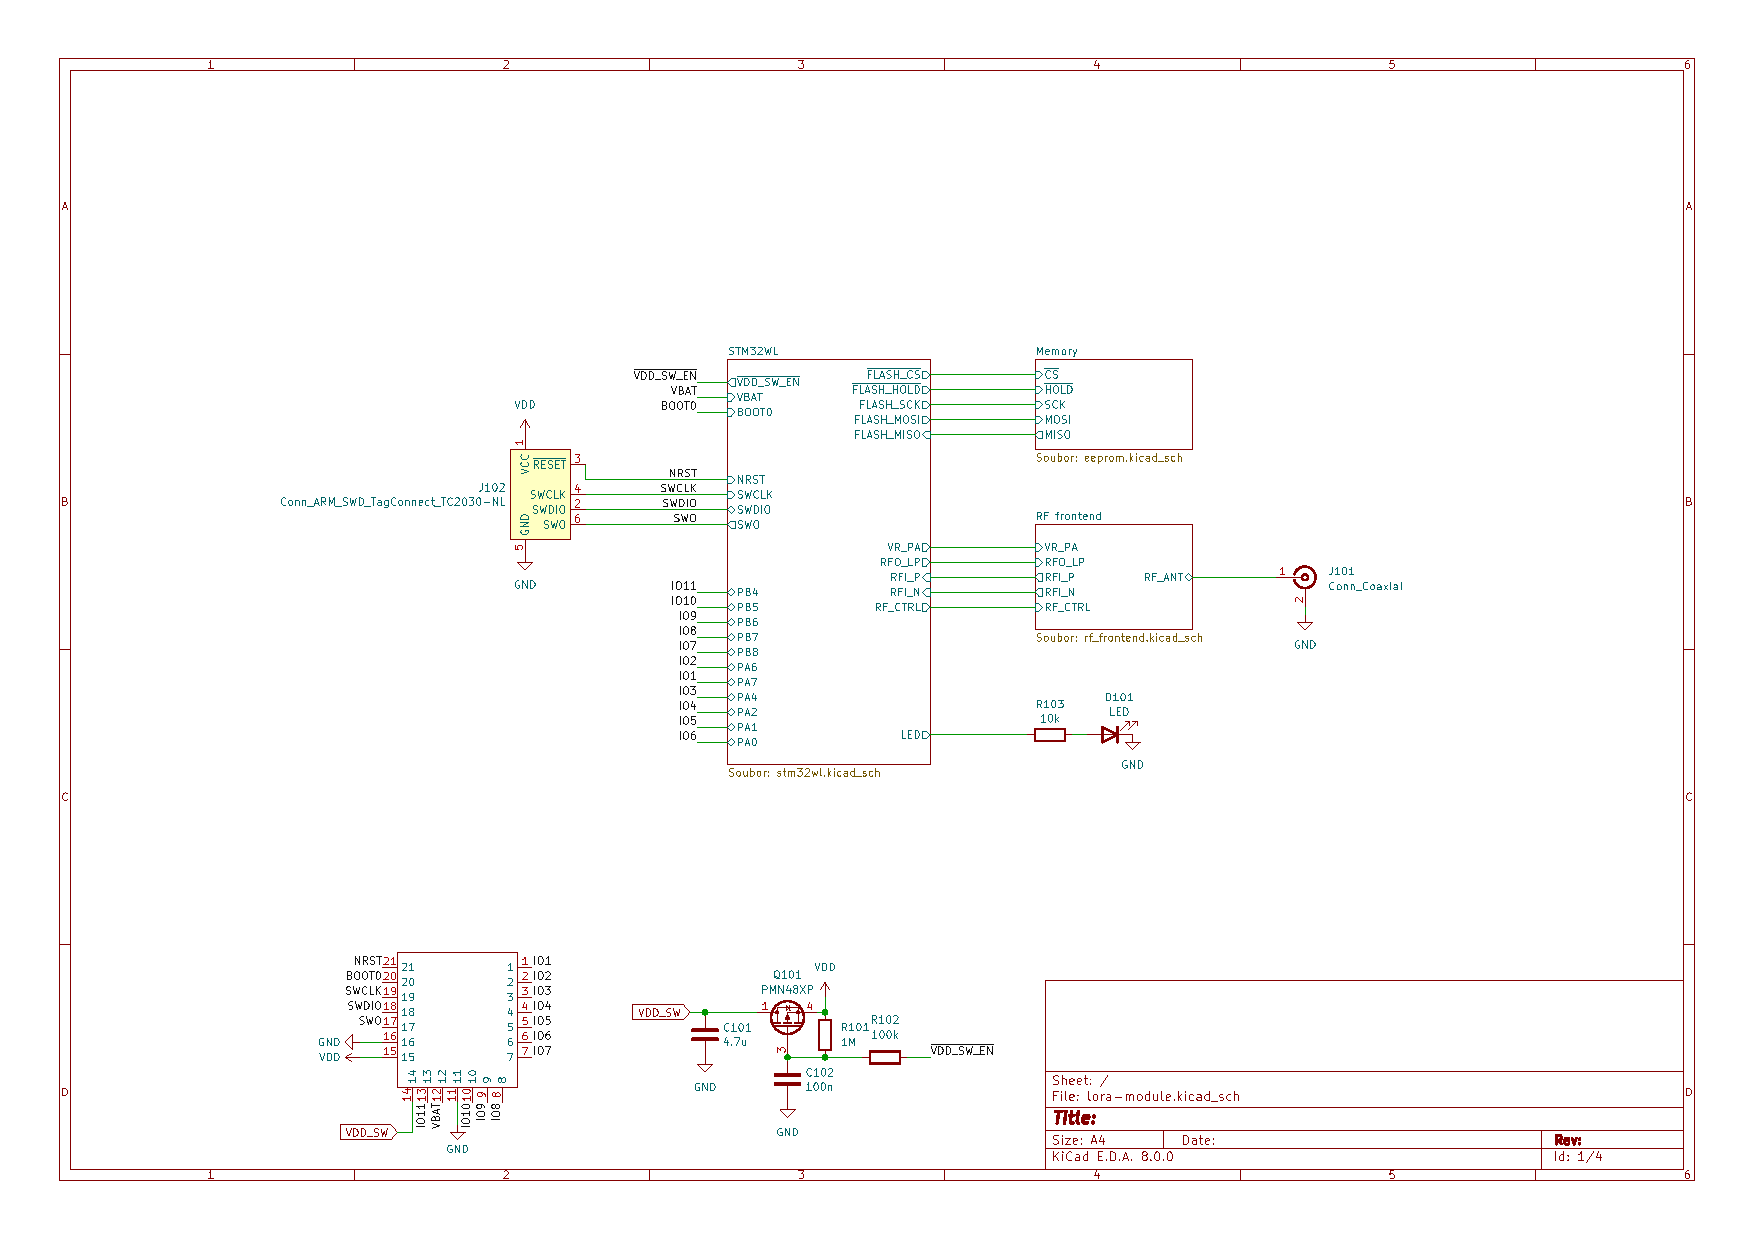
\includegraphics[page=1,angle=-90,width=\textwidth]{boards/v0.1/lora-module.pdf}
    \caption{\label{schematic:v0.1-1}Top level schematic sheet}
\end{figure}
\begin{figure}
    \includegraphics[page=2,angle=-90,width=\textwidth]{boards/v0.1/lora-module.pdf}
    \caption{\label{schematic:v0.1-2}STM32WLE5JC schematic sheet}
\end{figure}
\begin{figure}
    \includegraphics[page=3,angle=-90,width=\textwidth]{boards/v0.1/lora-module.pdf}
    \caption{\label{schematic:v0.1-3}RF frontend schematic sheet}
\end{figure}
\begin{figure}
    \includegraphics[page=4,angle=-90,width=\textwidth]{boards/v0.1/lora-module.pdf}
    \caption{\label{schematic:v0.1-4}Non-volatile memory schematic sheet}
\end{figure}

\begin{figure}
    \subfloat[Front layer]{\includesvg[width=.48\textwidth]{boards/v0.1/lora-module-F_Cu.svg}}\hfill
    \subfloat[Back layer]{\includesvg[width=.48\textwidth]{boards/v0.1/lora-module-B_Cu.svg}}\hfill
    \subfloat[Inner GND layer]{\includesvg[width=.48\textwidth]{boards/v0.1/lora-module-In1_Cu.svg}}\hfill
    \subfloat[Inner VCC layer]{\includesvg[width=.48\textwidth]{boards/v0.1/lora-module-In2_Cu.svg}}
    \caption{\label{board:v0.1}Module v0.1 PCB layer design}
\end{figure}

\begin{figure}
    \includesvg[width=\textwidth]{boards/v0.1/lora-module-F_Fab.svg}
    \caption{\label{board:v0.1-components}Module v0.1 component position reference}
\end{figure}

\chapter{\label{chapter:sensor-files}Soil Moisture Sensor Board Design Files}
%!TEX ROOT=main.tex

\begin{figure}[H]
    \subfloat[Front layer]{\includesvg[width=\textwidth]{boards/sensor/soil-sensor-F_Cu.svg}}\hfill
    \subfloat[Back layer]{\includesvg[width=\textwidth]{boards/sensor/soil-sensor-B_Cu.svg}}
    \caption{\label{board:sensor}Sensor PCB layer design}
\end{figure}

\begin{figure}[H]
    \subfloat[Electronics area]{\adjustbox{trim={0 0 15cm 0},clip,width=.6\textwidth}{\includesvg{boards/sensor/soil-sensor-F_Fab.svg}}}\hfil
    \subfloat[Tip area]{\adjustbox{trim={17.5cm 0 0 0},clip,width=.35\textwidth}{\includesvg{boards/sensor/soil-sensor-F_Fab.svg}}}
    \caption{\label{board:sensor-components}Sensor board component position reference}
\end{figure}

\begin{figure}
    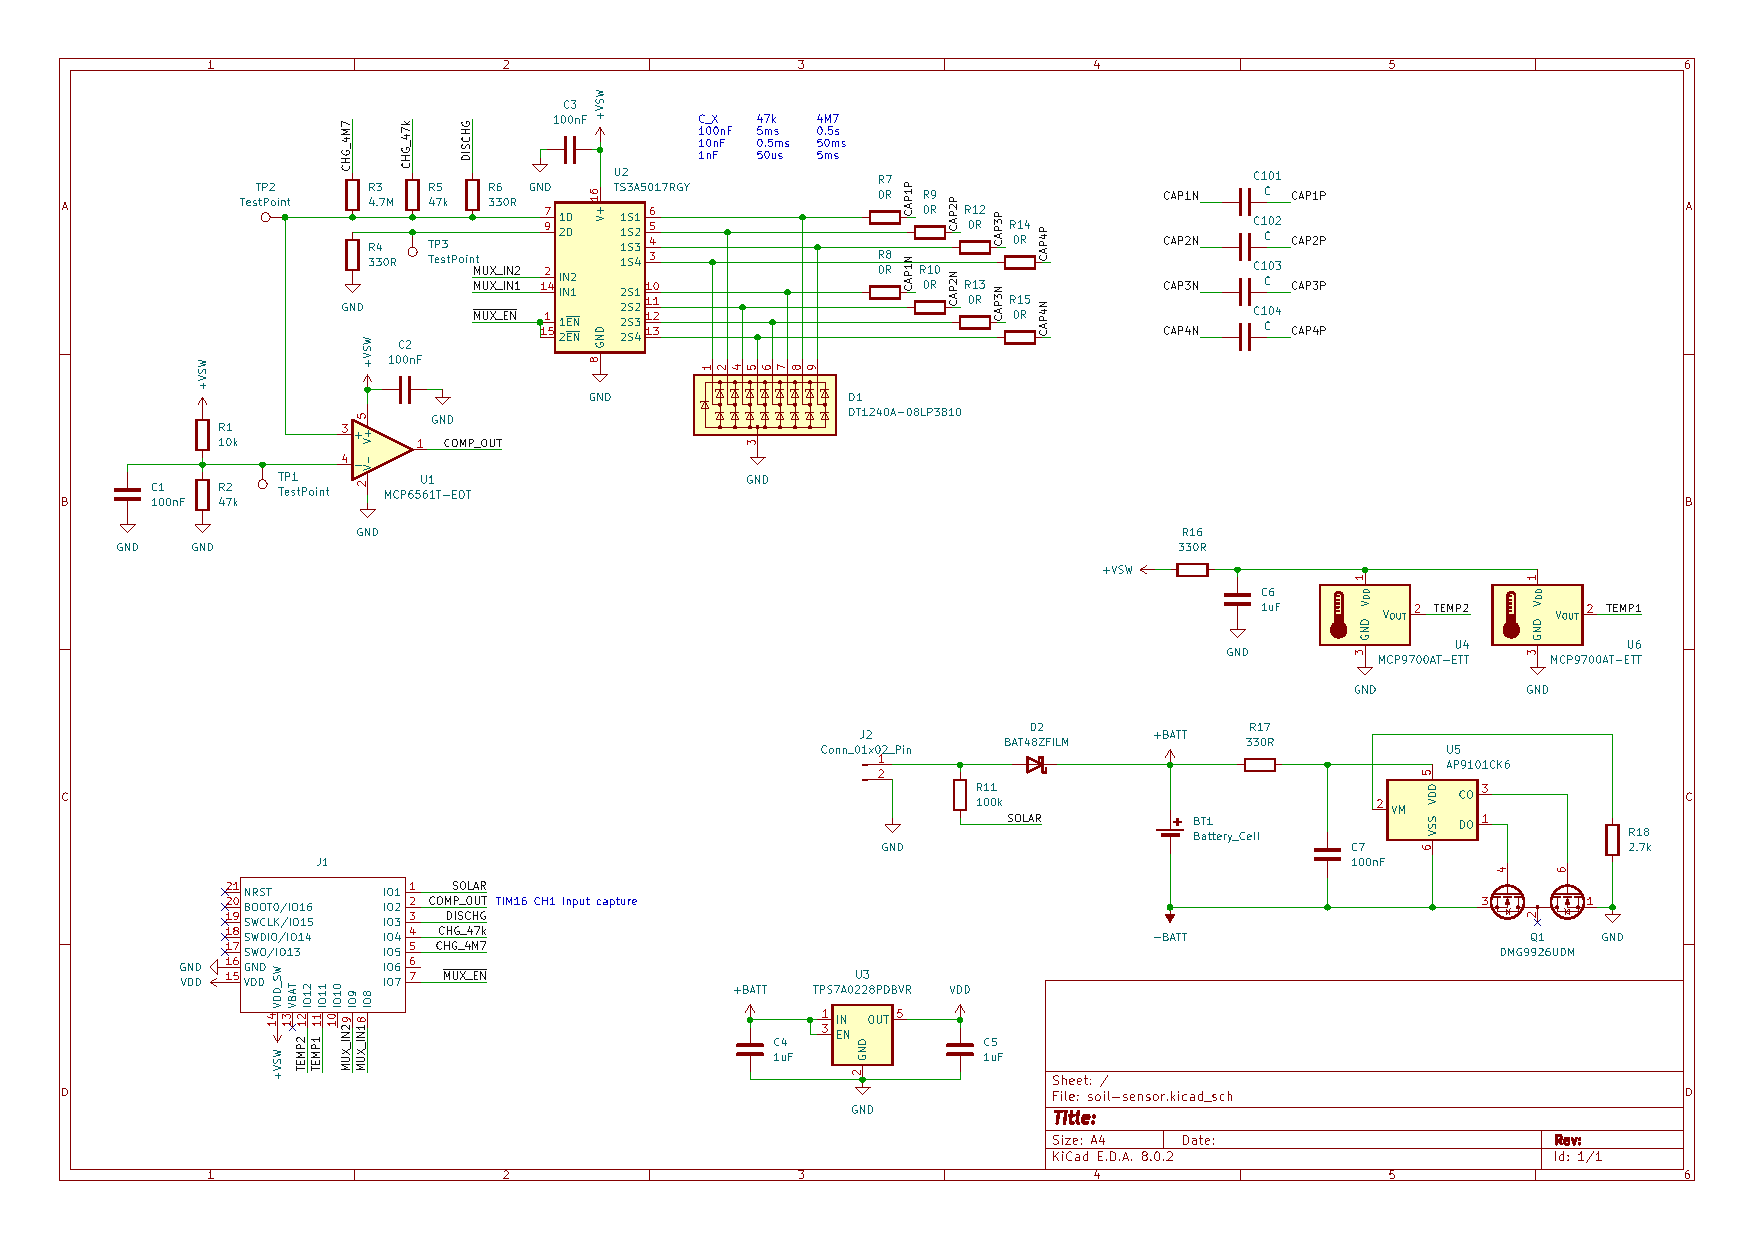
\includegraphics[page=1,angle=-90,width=\textwidth]{boards/sensor/soil-sensor.pdf}
    \caption{\label{schematic:sensor-1}Top level schematic sheet}
\end{figure}
\chapter{\label{chapter:more-range-test}Additional Data from the Range Test}
%!TEX ROOT=main.tex

The script that generated these graphs can be found at \link{https://github.com/manakjiri/bcs-thesis/blob/main/thesis/data/range/process.py}{thesis/data/range/process.py}.

\begin{figure}[H]
    \centering
    \subfloat[SF11]{\includesvg[width=\textwidth]{data/range/out/elevation-sf11.svg}} \hfil
    \subfloat[SF5]{\includesvg[width=\textwidth]{data/range/out/elevation-sf5.svg}}
    \caption{\label{fig:range-elevation}Graph of the range test locations, their distance from the pole with Nodes, and the elevation in the path of the signal. Black crosses signify the position of the antennae of each device for each spot number.}
\end{figure}

\begin{figure}[H]
    \centering
    \begin{minipage}[t]{.45\textwidth}
        \centering
        \vspace{0em}
        \begin{tabular}{|l|l|l|}
        \multicolumn{3}{c}{\textbf{SF11}} \\ \hline
        \textbf{Spot} & \textbf{Latitude} & \textbf{Longitude} \\ \hline
        0   & 50.0012006 & 14.5308962 \\ \hline
        1   & 50.0016874 & 14.5316496 \\ \hline
        2   & 50.0022362 & 14.5324151 \\ \hline
        3   & 50.0032967 & 14.5340917 \\ \hline
        4   & 50.0037838 & 14.5349146 \\ \hline
        5   & 50.0047636 & 14.5365683 \\ \hline
        6   & 50.0054468 & 14.5377137 \\ \hline
        7   & 50.0058617 & 14.5390798 \\ \hline
        8   & 50.0060974 & 14.5406886 \\ \hline
        9   & 50.0063041 & 14.5424961 \\ \hline
        10  & 50.0066088 & 14.5446115 \\ \hline
        11  & 50.0066739 & 14.5449186 \\ \hline
        \end{tabular}
    \end{minipage}
    \begin{minipage}[t]{.45\textwidth}
        \centering
        \vspace{0em}
        \begin{tabular}{|l|l|l|}
        \multicolumn{3}{c}{\textbf{SF5}} \\ \hline
        \textbf{Spot} & \textbf{Latitude} & \textbf{Longitude} \\ \hline
        0   & 50.0012006 & 14.5308962 \\ \hline
        1   & 50.0016885 & 14.5316117 \\ \hline
        2   & 50.0022075 & 14.5323917 \\ \hline
        3   & 50.0032262 & 14.5339823 \\ \hline
        4   & 50.0038245 & 14.5349764 \\ \hline
        5   & 50.0046297 & 14.5363408 \\ \hline
        6   & 50.0051263 & 14.5371679 \\ \hline
        7   & 50.0060381 & 14.5402405 \\ \hline
        8   & 50.0063383 & 14.5425206 \\ \hline
        9   & 50.0067234 & 14.5456749 \\ \hline
        \end{tabular}
    \end{minipage}
    \caption{Precise coordinates of each spot in the range test.}
\end{figure}

\begin{figure}[H]
    \centering
    \subfloat[SF11-FAR1]{\includesvg[width=\textwidth]{data/range/out/elevation-sf11-far1.svg}} \hfil
    \subfloat[SF11-FAR2]{\includesvg[width=\textwidth]{data/range/out/elevation-sf11-far2.svg}}
    \caption{\label{fig:range-elevation-far}Graph of the range test locations, their distance from the pole with Nodes, and the elevation in the path of the signal. Black crosses signify the position of the antennae of each device for each spot number.}
\end{figure}
\end{appendices}

\bibliographystyle{plainurl}
\bibliography{main.bib}

\end{document}